\chapter{Results and discussion}
\label{chap:results}
%\section{Number of simulations}
%The  algorithm makes usage of randomly distributed users causing each simulation to be difference. The results are based on average values over multiple simulations. It is therefore important knowing how mush simulations is required in order to become a converged average. This is done by using an example scenario which details can be found in table \ref{table:configForNumberOfUsers}. The most important parameters
%investigated in the different scenarios are $SAR_{10g}$, power consumption and user coverage. Therefore, the cummulative avarage of each investigated value is plotted in function of number of simulations.
\iffalse %remove to reanable section (dont forget fi little further)
\begin{table}[!htb]
\centering
  \begin{tabular}{|l|l|}
  \hline
  Parameter               & value          \\   \hline 
  number of users               & 40            \\ 
  facilityCapacity                    & 20           \\ 
  fixedFlyHeight               & 100           \\ 
  optimization strategy               & power consumption optimized           \\ 
  \hline
  \end{tabular}
  \caption{Overview of the configuration.}
  \label{table:confOverviewScenario2}
\end{table}

The number of simulations has a direct influence on the runtime. Certain configurations take a considerable amount of runtime (expessed in hours). This is because of the
exponential time complexity. The deployment tool with $n$ users, will need to calculate $n$ times the path loss between $n$ drones and $n$ users and thereafter $n/2$ times between
each user. Thereafter, each user will have to be connected to the best possible \gls{UABS} and each user is therefore required to consider multiple \gls{UABS}s.

\begin{figure}[th!]
  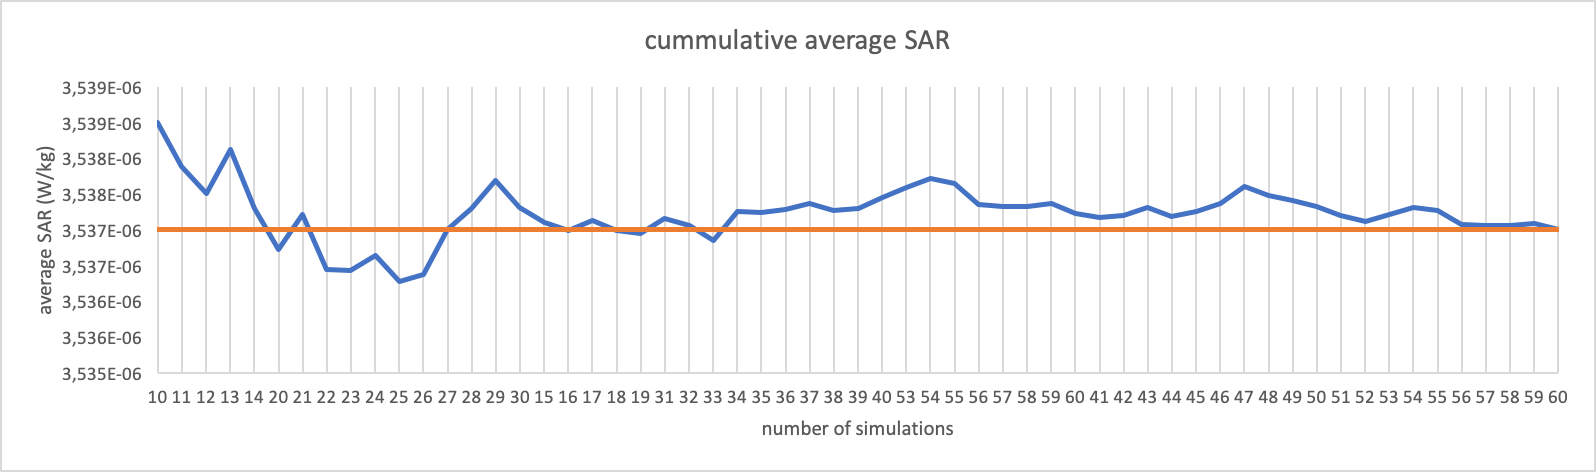
\includegraphics[width=\textwidth]{../results/numberOfSim/sarvssim.png}
  \caption{Total SAR versus.}
  \label{fig:fhsar}
\end{figure}
\begin{figure}[th!]
  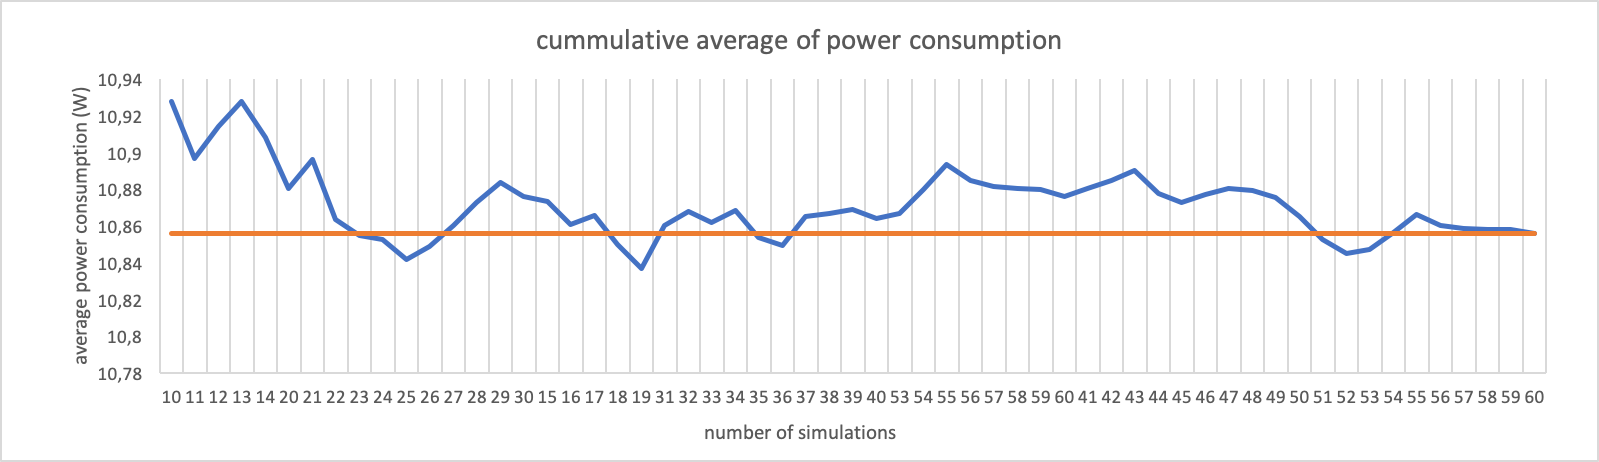
\includegraphics[width=\textwidth]{../results/numberOfSim/pcvssim.png}
  \caption{General design of a microstrip antenna.}
  \label{fig:fhsar}
\end{figure}
\begin{figure}[th!]
  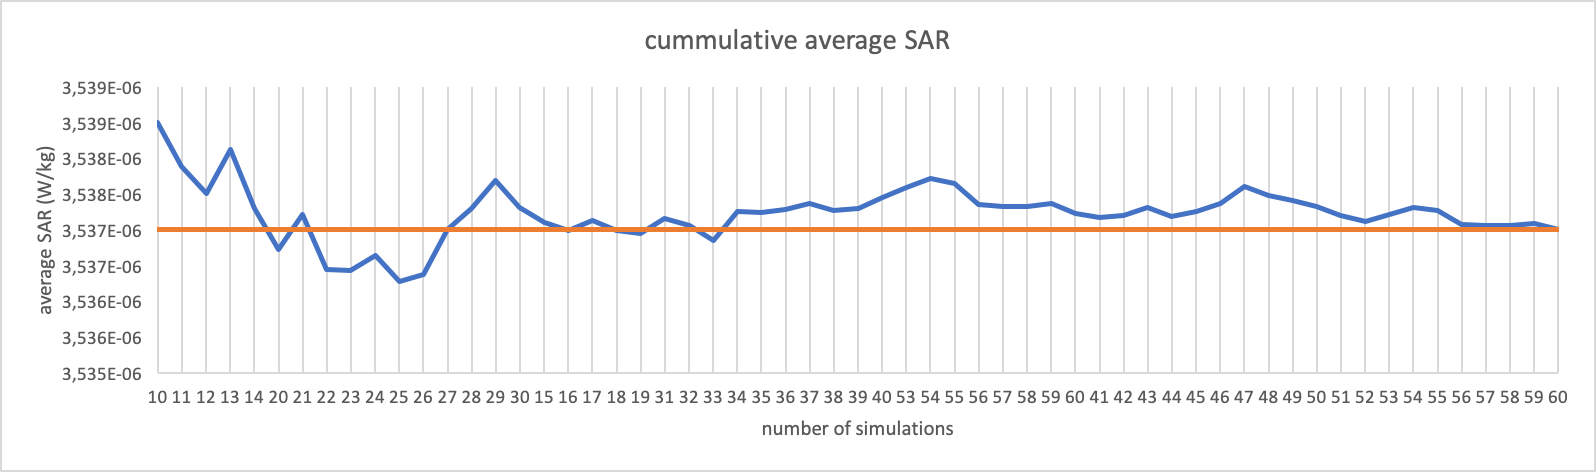
\includegraphics[width=\textwidth]{../results/numberOfSim/sarvssim.png}
  \caption{General design of a microstrip antenna.}
  \label{fig:fhsar}
\end{figure}
\fi %remove to reanable section
%%%%%%%%%%%%%%%%%%%%%%%%%%%%%%%%%%%%%%%%%%%%%%%%%%%%%%%%%%%%%%%%%%%%%%%%%%%%%%%%%%%%%%%%%%%%%%%%%%%%%%%%%%%%%%%%%%%%%%%%%%%%%%%%%%%%
\section{Scenario 1: One User and One Drone}
The network contains only one user for this scenario. This means that there is only one location possible for the drone which is just above 
the user. This section will investigate minimal required transmission power and SAR values from different sources.
\textcolor{red}{power consumption te doen}

\subsection{The influence of the maximum transmission power}
\gls{LTE} makes usages of power control meaning that no more power will be used then strictly necessary. The actual 
transmit power $P_{tx}$ therefore ranges between 0 and the maximum input power. $P_{tx}$ is zero when the \gls{UABS} doesn't cover anybody.
Increasing the maximum transmission power won't influence the power consumption or $SAR_{10g}$ because the \gls{UABS} won't use more
then strictly required. It is therefore more useful to match the actual transmission power against a variable flying height. Figure \ref{fig:ptxfh}
shows a logarithmic  relationship showing that $P_{tx}$ increases fast at low altitude but slows down at higher altitudes. 

Figure \ref{fig:ptxfh} shows the minimal required energy by an \gls{isotropicradiator} in order to reach the user just below him.
As already discussed in \ref{sec:s1}, the user is outdoor and just below the \gls{UABS}. There is thus a free line-of-sight between both
radiators. It is clear  from figure \ref{fig:ptxfh} that a step function is achieved because multiple flying heights correspond to the same transmission power.
When the flying height increases, so does the path loss. \gls{LTE} tries to counteract this by increasing the power level. Each time 
the path loss becomes too high, the power level of the antenna increases with one dBm. Doing so, decreases path loss allowing the antenna to reach
the user again. 

After a jump in the step function, there is an overestimation meaning the input power increased more then necessary. So multiple flying heights correspond with the same $P_{tx}$.
dBm has a logarithmic scale meaning that while 10 dBm equals 10 mW, 20 dBm equals 100 mW. This explains why the black lines become longer at higher flying altitudes.
Each time the power level increases with one dBm, the overestimation becomes larger.

If the tool would make usage of smaller step size, a more continuous 
logarithmic function would be achieve. This would however worsen the time complexity because increasing the power level to exceed the path loss
would happen in much smaller steps. The red line indicates the default maximum transmission power used during simulations. 
In a free line-of-sight scenario with only one user, a \gls{UABS} can fly up to 387 meters before losing connection.

This scenario is investigated with a microstrip patch antenna using power consumption optimization
and however an \gls{isotropicradiator} doesn't have any attenuation while a microstrip patch antenna does, these parameters does not matter.
This is because the user is positioned in the perfect center of the main beam where there is 
no attenuation in either cases. Also the optimization won't make a difference. The goal of the  strategy is to decide which drone is most suitable for which
users. Since there is only one user and one possible position for the drone, both optimization strategies behave identical.

\begin{figure}[h!]
  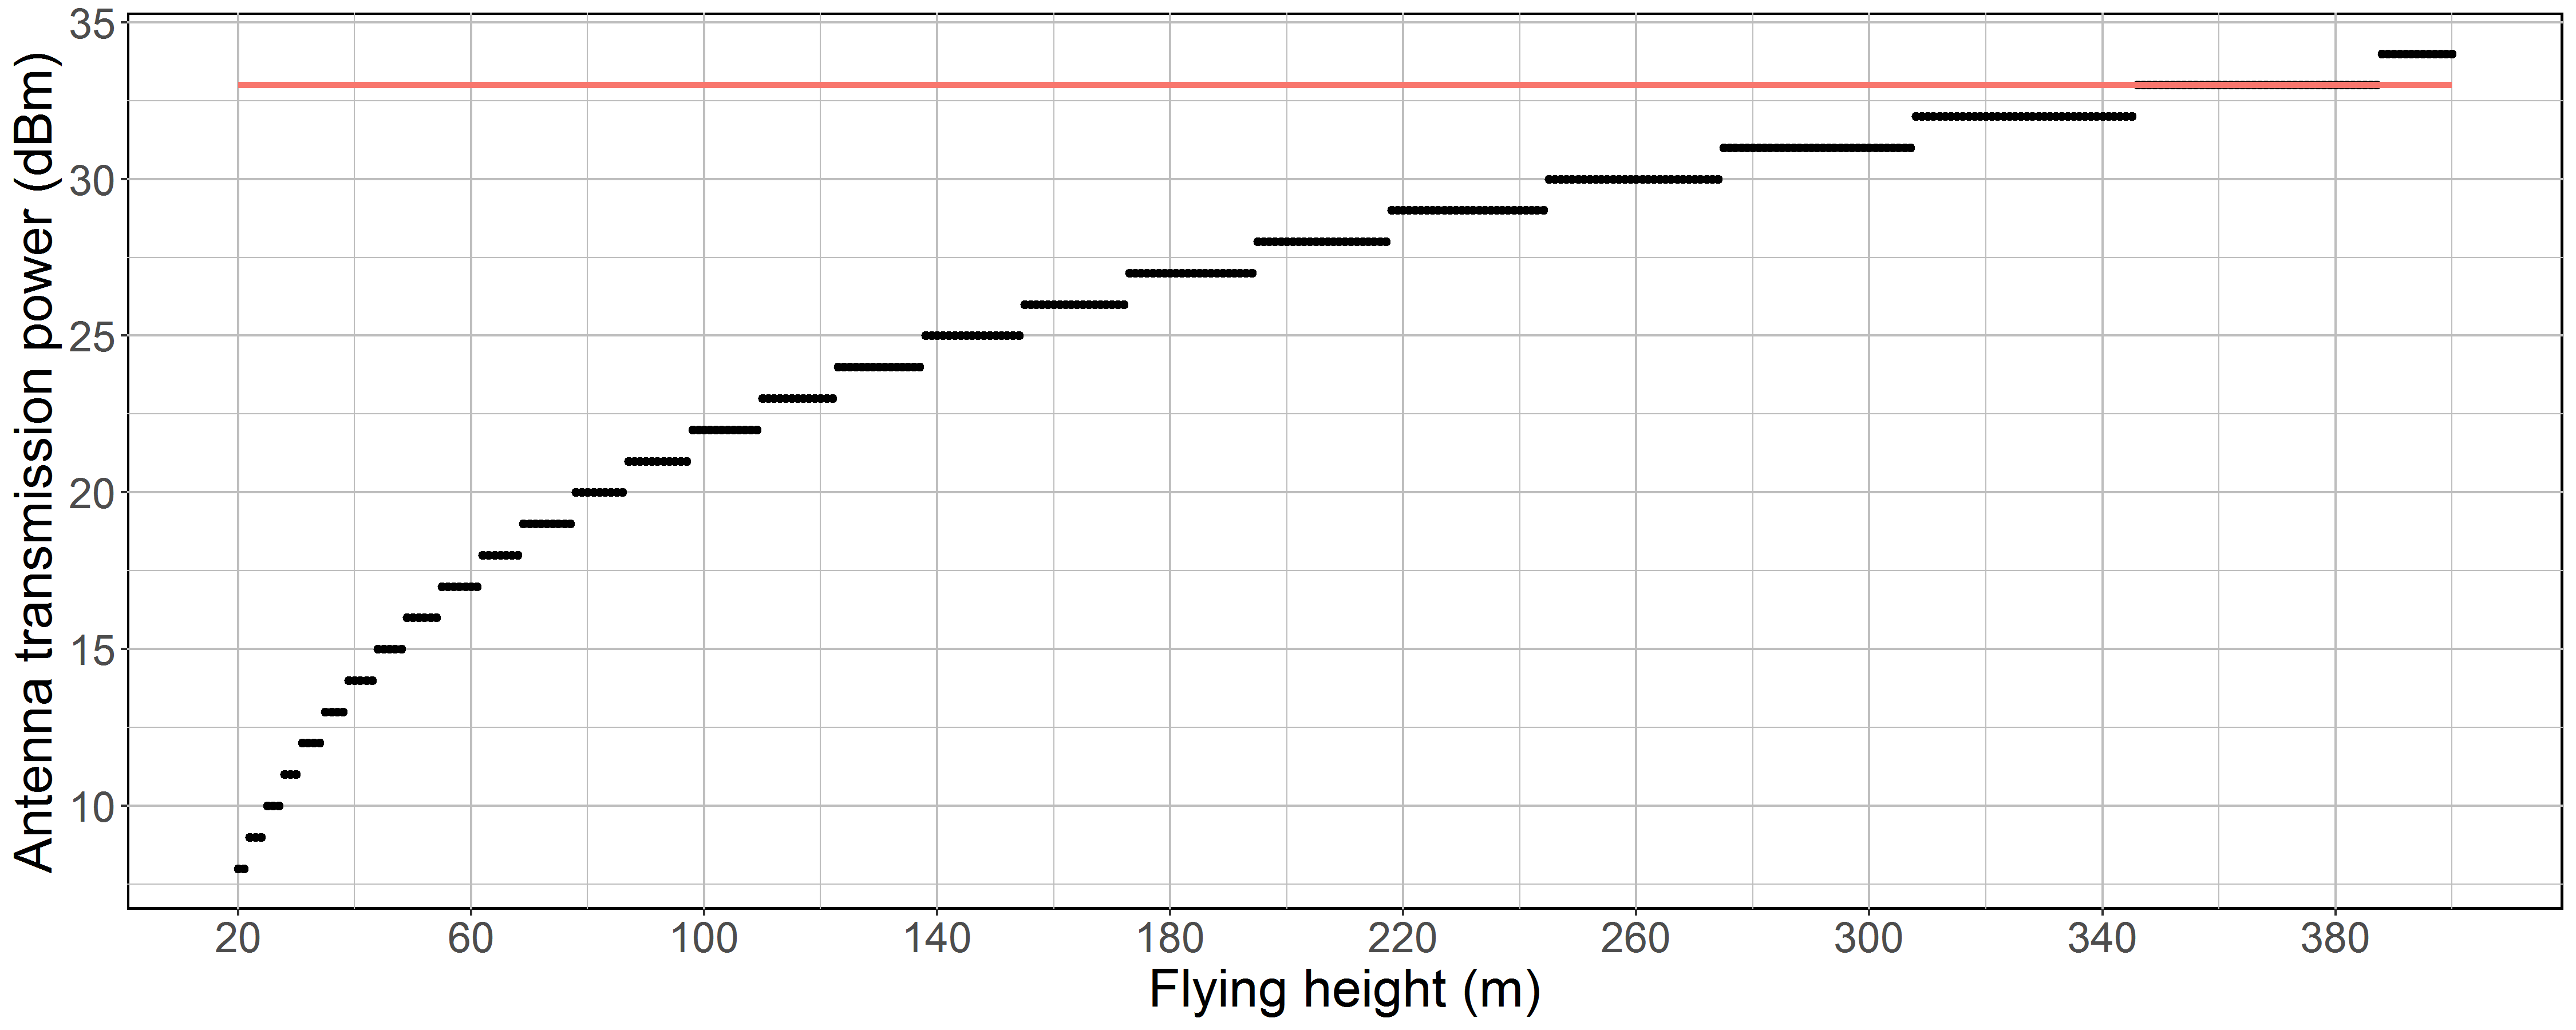
\includegraphics[width=\textwidth]{../results/s1/ptx.png}
  \caption{Minimal required transmission power by the antenna to reach the ground just below him. The red line shows the default maximum transmission power.}
  \label{fig:ptxfh}
\end{figure}

\subsection{Influence of the flying height}
\label{sub:senario1_influenceOfFlyHeight}

This section investigates how the flying height of a \gls{UABS} influence $SAR_{10g}$ and power consumption. In figure \ref{fig:s1_fhsar}
becomes clear that with an increasing flying height, the specific absorption rate grows exponentially 
which is also the case for the power consumption in figure \ref{fig:pcsar}.

Figure \ref{fig:s1_fhsar} shows represents the induced electromagnetic radiation for our user 
and shows that for low flying drones, \gls{UABS}s are the main source of electromagnetic radiatio which is indicated with the green line.
This changes around 80 meters where \gls{UL} electromagnetic radiation of the \gls{UE} (indicated with the red line)
exceeds \gls{DL} radiation in order to still be able to reach the high flying \gls{UABS}s.

The green line (representing the $SAR^{basestation}_{10g}$) shows the same discontinue 
behaviour from in figure \ref{fig:ptxfh}. As explained before, \gls{LTE} makes usage of power control. Meaning that the power transmission only increases when paht loss 
increases up to the point where the power level exceeds its maximum after which connection is lost completely and exposure drops to zero. 
This behaviour causes the electromagnetic radiation experienced by the user to be almost constant. The slightly visible variation in the green line
has the same reason as why figure \ref{fig:ptxfh} shows a step function. The green line can be simplified to a constant linear line.
This means that 
the electromagnetic radiation before it was converted into  \gls{UABS} using the formulas from section \ref{sub:convertDLtosarwb} was 
also constant because of power control.
 The exposure is in other words a constant fraction of power and distance like shown in equation \ref{eq:exposureBasicFormula}.

\begin{equation}
\vec{E} (V/m) = \frac{\Delta U (V) }{\Delta x (m)}
\label{eq:exposureBasicFormula}
\end{equation}

Figure \ref{fig:s1_fhsar} doesn't show radiation from neighbours, because there are non present in this scenario. Finally, all these values are added as explained in formula
\ref{eq:overallSARwb} and indicated with the blue line. 
\begin{figure}[th!]
  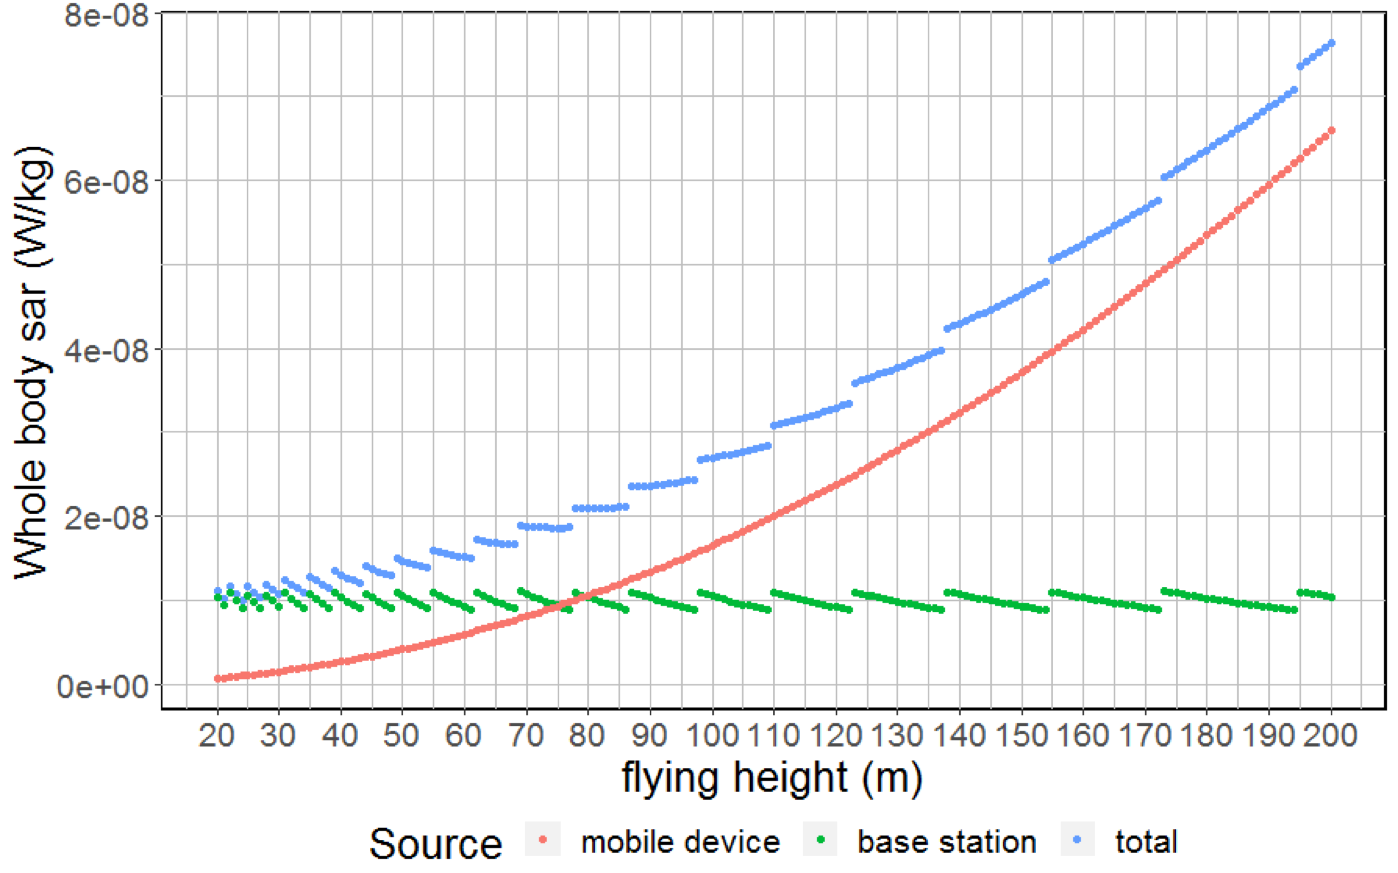
\includegraphics[width=\textwidth]{../results/s1/fhvssar2.png}
  \caption{How SAR values from different sources are influenced by different flying altitudes.}
  \label{fig:s1_fhsar}
\end{figure}

\textcolor{red}{power consumption te doen}
%%%%%%%%%%%%%%%%%%%%%%%%%%%%%%%%%%%%%%%%%%%%%%%%%%%%%%%%%%%%%%%%%%%%%%%%%%%%%%%%%%%%%%%%%%%%%%%%%%%%%%%%%%%%%
\section{Scenario 2: Increased Traffic}

This scenario has just like the previous scenario only one drone. However, more users will be present in the network.
First, a variable flying altitude is investigated for a fixed number of 224 users. 
Secondly, the flying height is set to 100 metres with a variable number of users.
When designing the network, there will be as much possible drone locations as there are users in the network and the tool
will consider all of them. It's only when the programme is finished, that one drone remains.

\subsection{Influence of the flying altitude}
This scenario investigates how the network consisting of one \gls{UABS} behaves when applied on an ordinary day during rush hour. 
On average, 224 active users are distributed uniformly over the city center of Ghent. 
Chart \ref{fig:s2fhvsdl} shows how the downlink exposure is clearly influenced by the flying height of the \gls{UABS}. 
This is because if a drone flies higher, there is less penetration loss from obstructing buildings.

A power consumption optimized network with an \gls{EIRP} antenna (green) has the highest exposure. 
This is logical when comparing with an EIRP antenna in an exposure optimized network (red). 
However, when looking at chart \ref{fig:s2fhvspc}, the power consumption in a power consumption optimized network is worse 
than in an exposure optimized network. To understand this, the behavior of the deployment tool needs to be understood first. 
A power consumption optimized network will result in few high powered \gls{UABS}s because increasing the input power of an antenna cost 
less then activating a new  drone. Likewise, an exposure optimized network 
generates a lot of low powered \gls{UABS}s because the lower the antenna's power, the lower the exposure. This has the consequence that the cover radius 
is less and therefore requiring more drones and powering up more drones cost more energy.
When only limited amount of \gls{UABS}s are available, 
like only one in this scenario, the tool will only keep \gls{UABS}s which cover most of the users. 
Therefore, is the power consumption in a power consumption optimized network way higher. 


\begin{figure}[h!]
  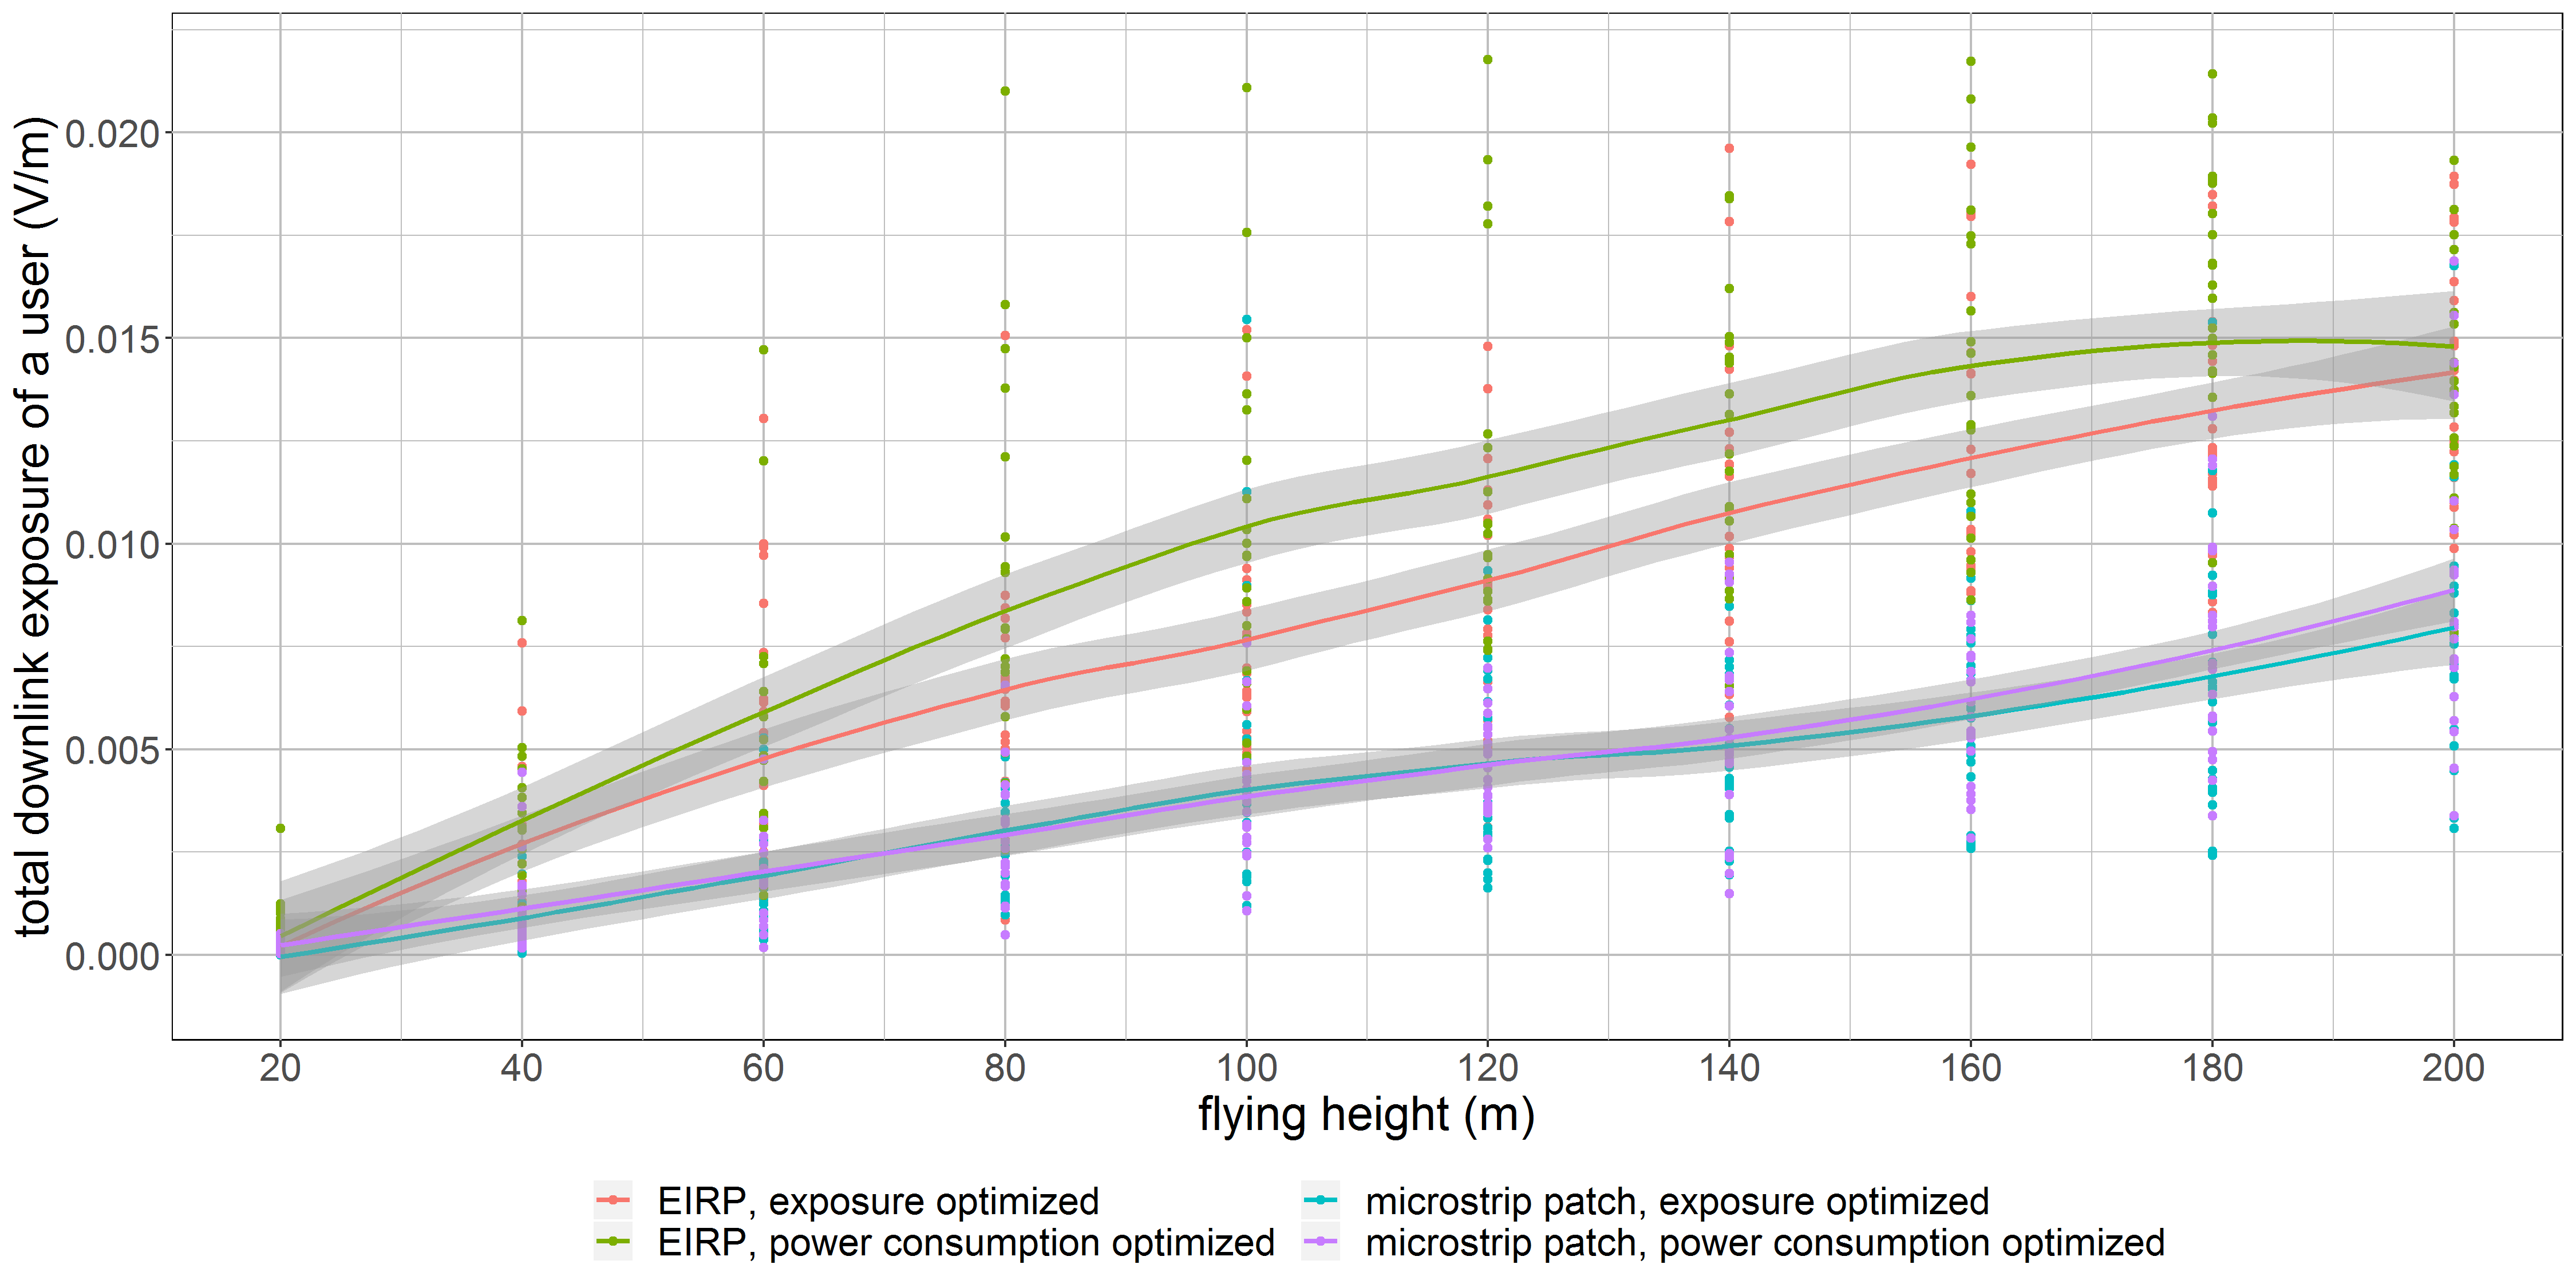
\includegraphics[width=\textwidth]{../results/s2/fhvsdl.png}
  \caption{The influence of the flying height on the weighted average downlink exposure of users in the network.}
  \label{fig:s2fhvsdl}
\end{figure}

\begin{figure}[bh!]
  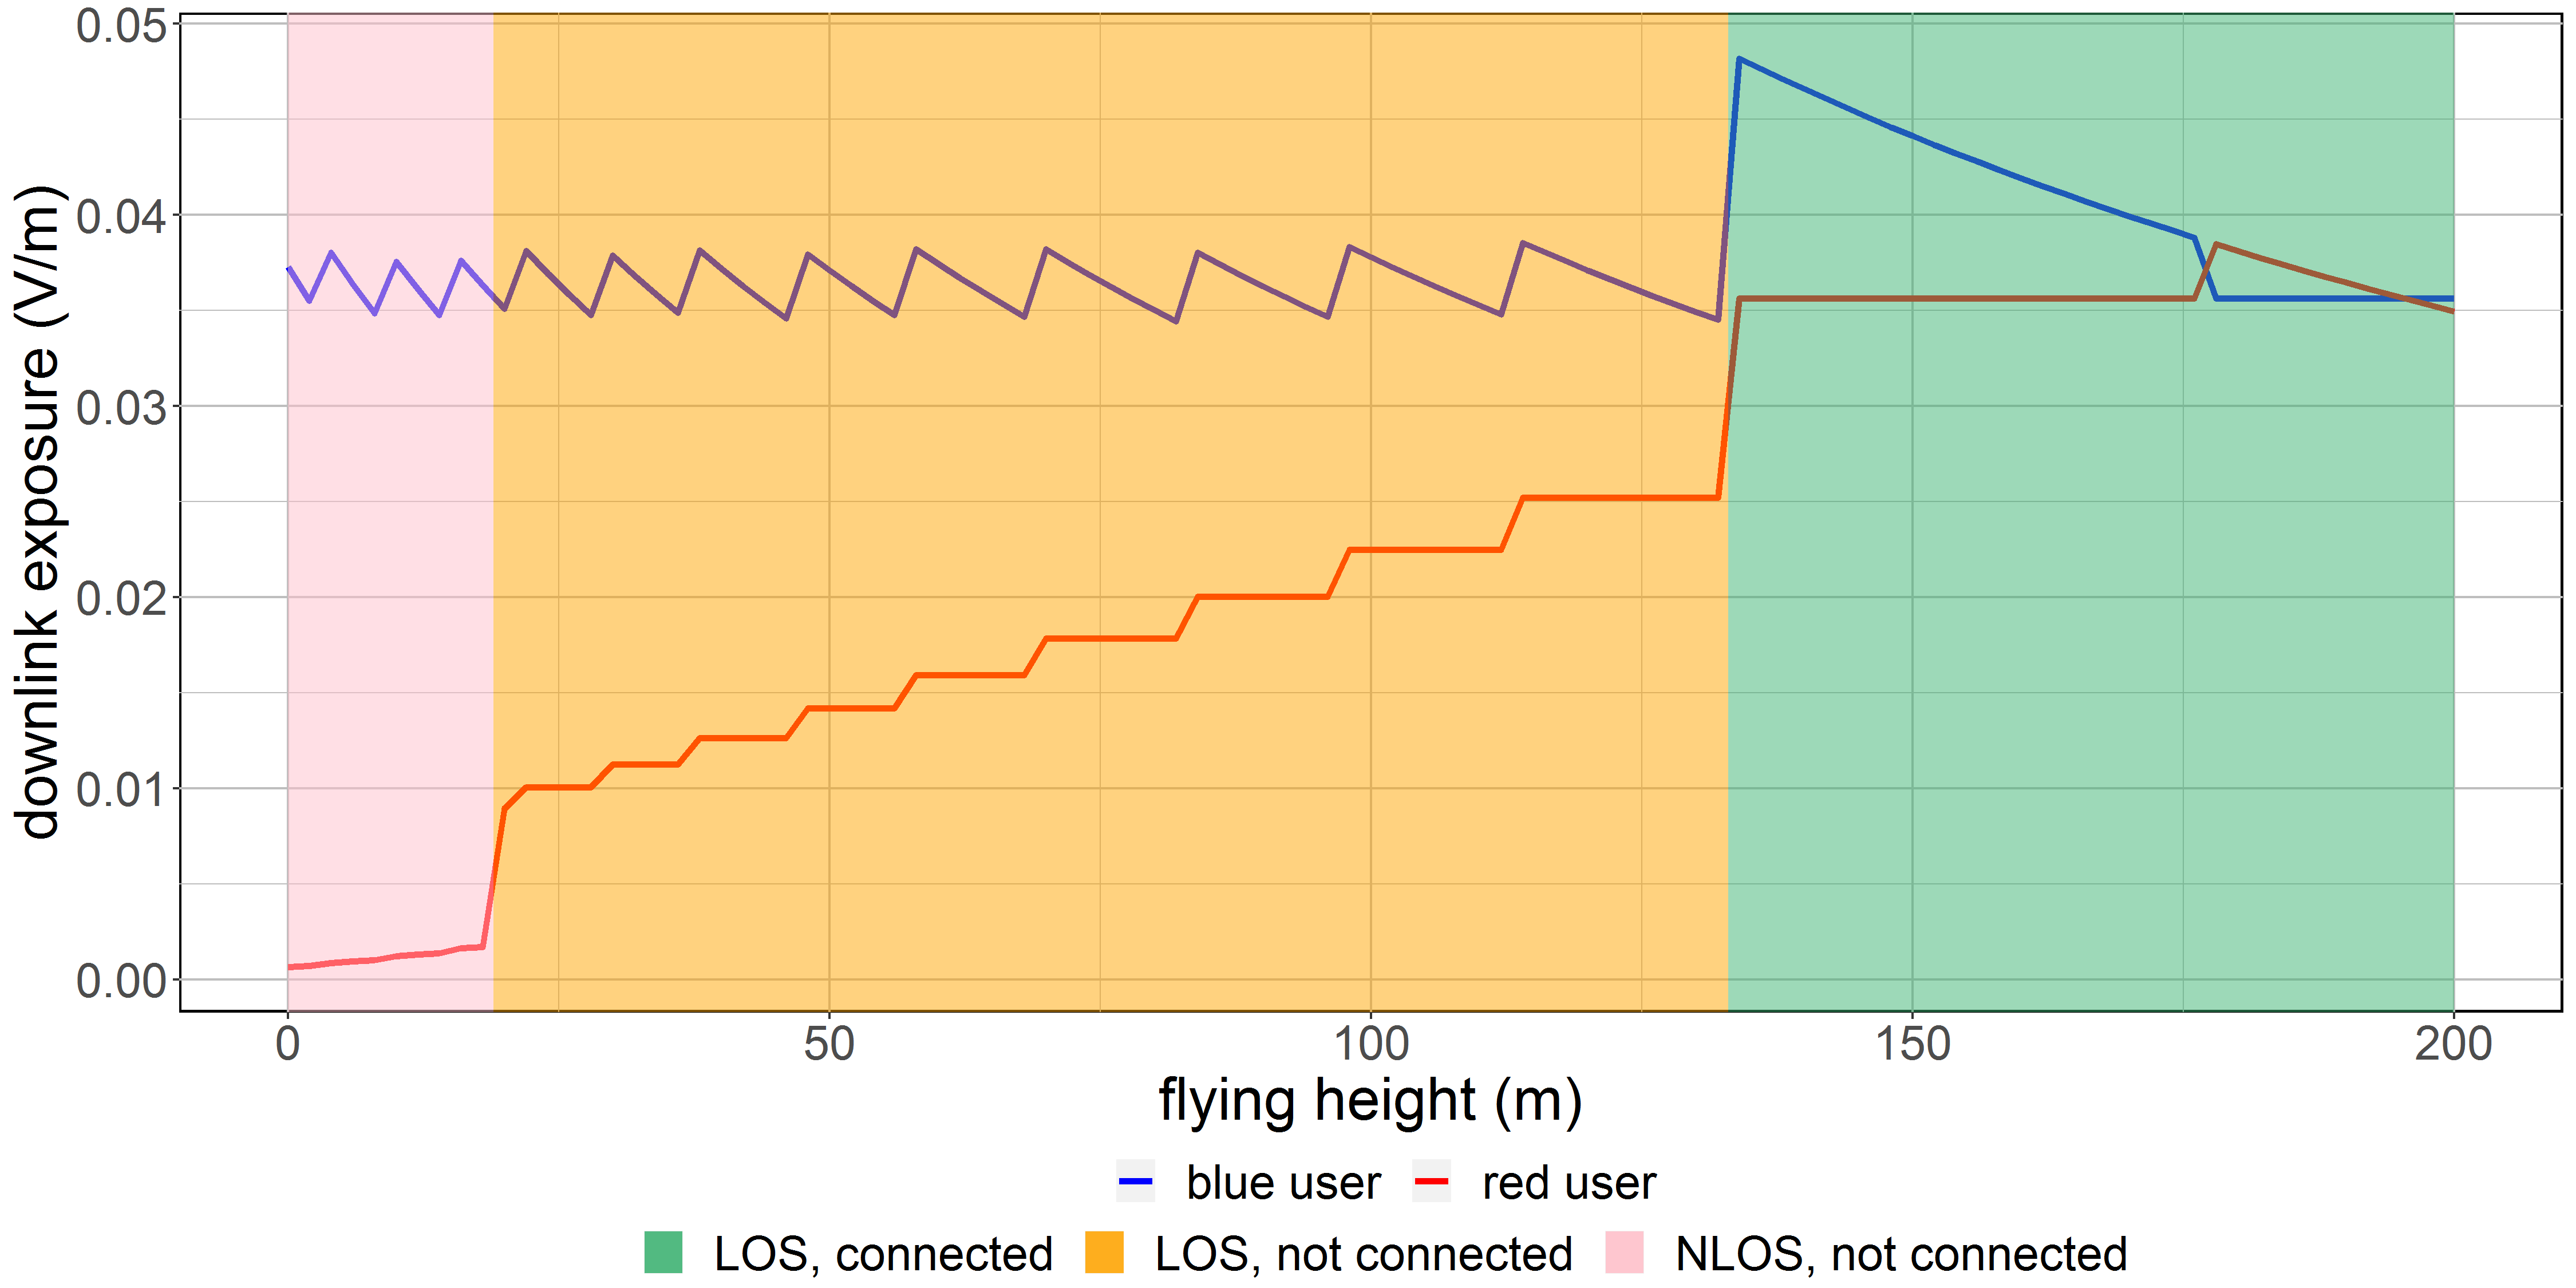
\includegraphics[width=\textwidth]{../results/s2/prove.png}
  \caption{Scenario 2 with only 2 users. The coloured areas are only applicable for the orange user. The blue user is connected during the entire time.}
  \label{fig:prove}
\end{figure}


\begin{wrapfigure}{r}{0.49\textwidth}
  \begin{center}
    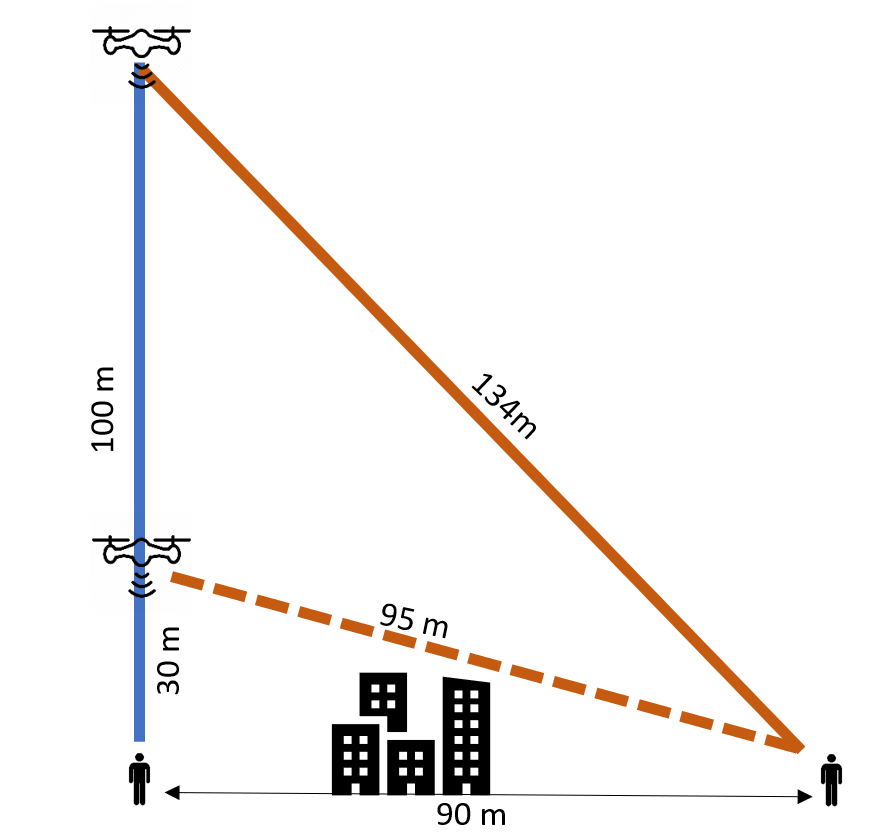
\includegraphics[width=0.48\textwidth]{../results/s2/proveScenario.png}
  \end{center}
  \caption{Schematic overview of scenario 2 with only 2 users.}
  \label{fig:schematicprove}
\end{wrapfigure}

\newpage
The correctness of figure \ref{fig:s2fhvsdl} is proven with figure \ref{fig:prove} by investigating the scenario with only two users. The two users who 
will be referred to by `red' and `blue' user are 90 metres separated from each other with a building between them.
Scenario 1 already explained that the charts can be simplified and the blue line from fig. \ref{fig:prove} remains in fact constant between the zero and 130 metres.
The chart shows that the \gls{UABS} is positioned above the blue user. The orange user is in \gls{NLOS} as long as the \gls{UABS} remains below 20 metres.

Once the \gls{UABS} increases it flying altitude, the orange user becomes into \gls{LOS} but still remains uncovered. This is because the tool initially locate a possible 
\gls{UABS} above each user and thereafter performs a  fitness function. The applied fitness function must have decided that it is better to connect 
each user to the \gls{UABS} above him. At a final state, the tool check whether the number of online drones does not exceed the capacity of the facility
which is here the case. The tool therefore deactivates one \gls{UABS} causing the orange user to be uncovered. One could argue that the 
the orange user should be connected to the online drone who is only 90 metres away. This would however require the online drone to increase his power consumption which 
would make the decisions made by the optimization strategy obsolete.

When the drone flies higher, the difference in distance between both users and the base station decreases. In other words, the Pythagorean theorem shows that when the flying height of the 
\gls{UABS} increases, the distance with the blue user increases faster compared to the distance between that same \gls{UABS} and the orange user. This is also illustrated in figure \ref{fig:schematicprove}.

At 130 metres, the tool decides to connect both users to the same UABS. Therefore, it increases it's power consumption so the orange user would  have the minimal 
required electromagnetic exposure. This has of course a negative influence for the blue user who is way closer and experience now a much higher exposure level.

Around 180 metres, the  orange and blue line switch. This is because the drone switches position. As explained before, the tool assigns two possible drones, one above 
each user. The tool must have decided that connecting both users to the other drones improves the fitness function of the entire network even though that difference might be 
very little.



\begin{figure}[h!]
  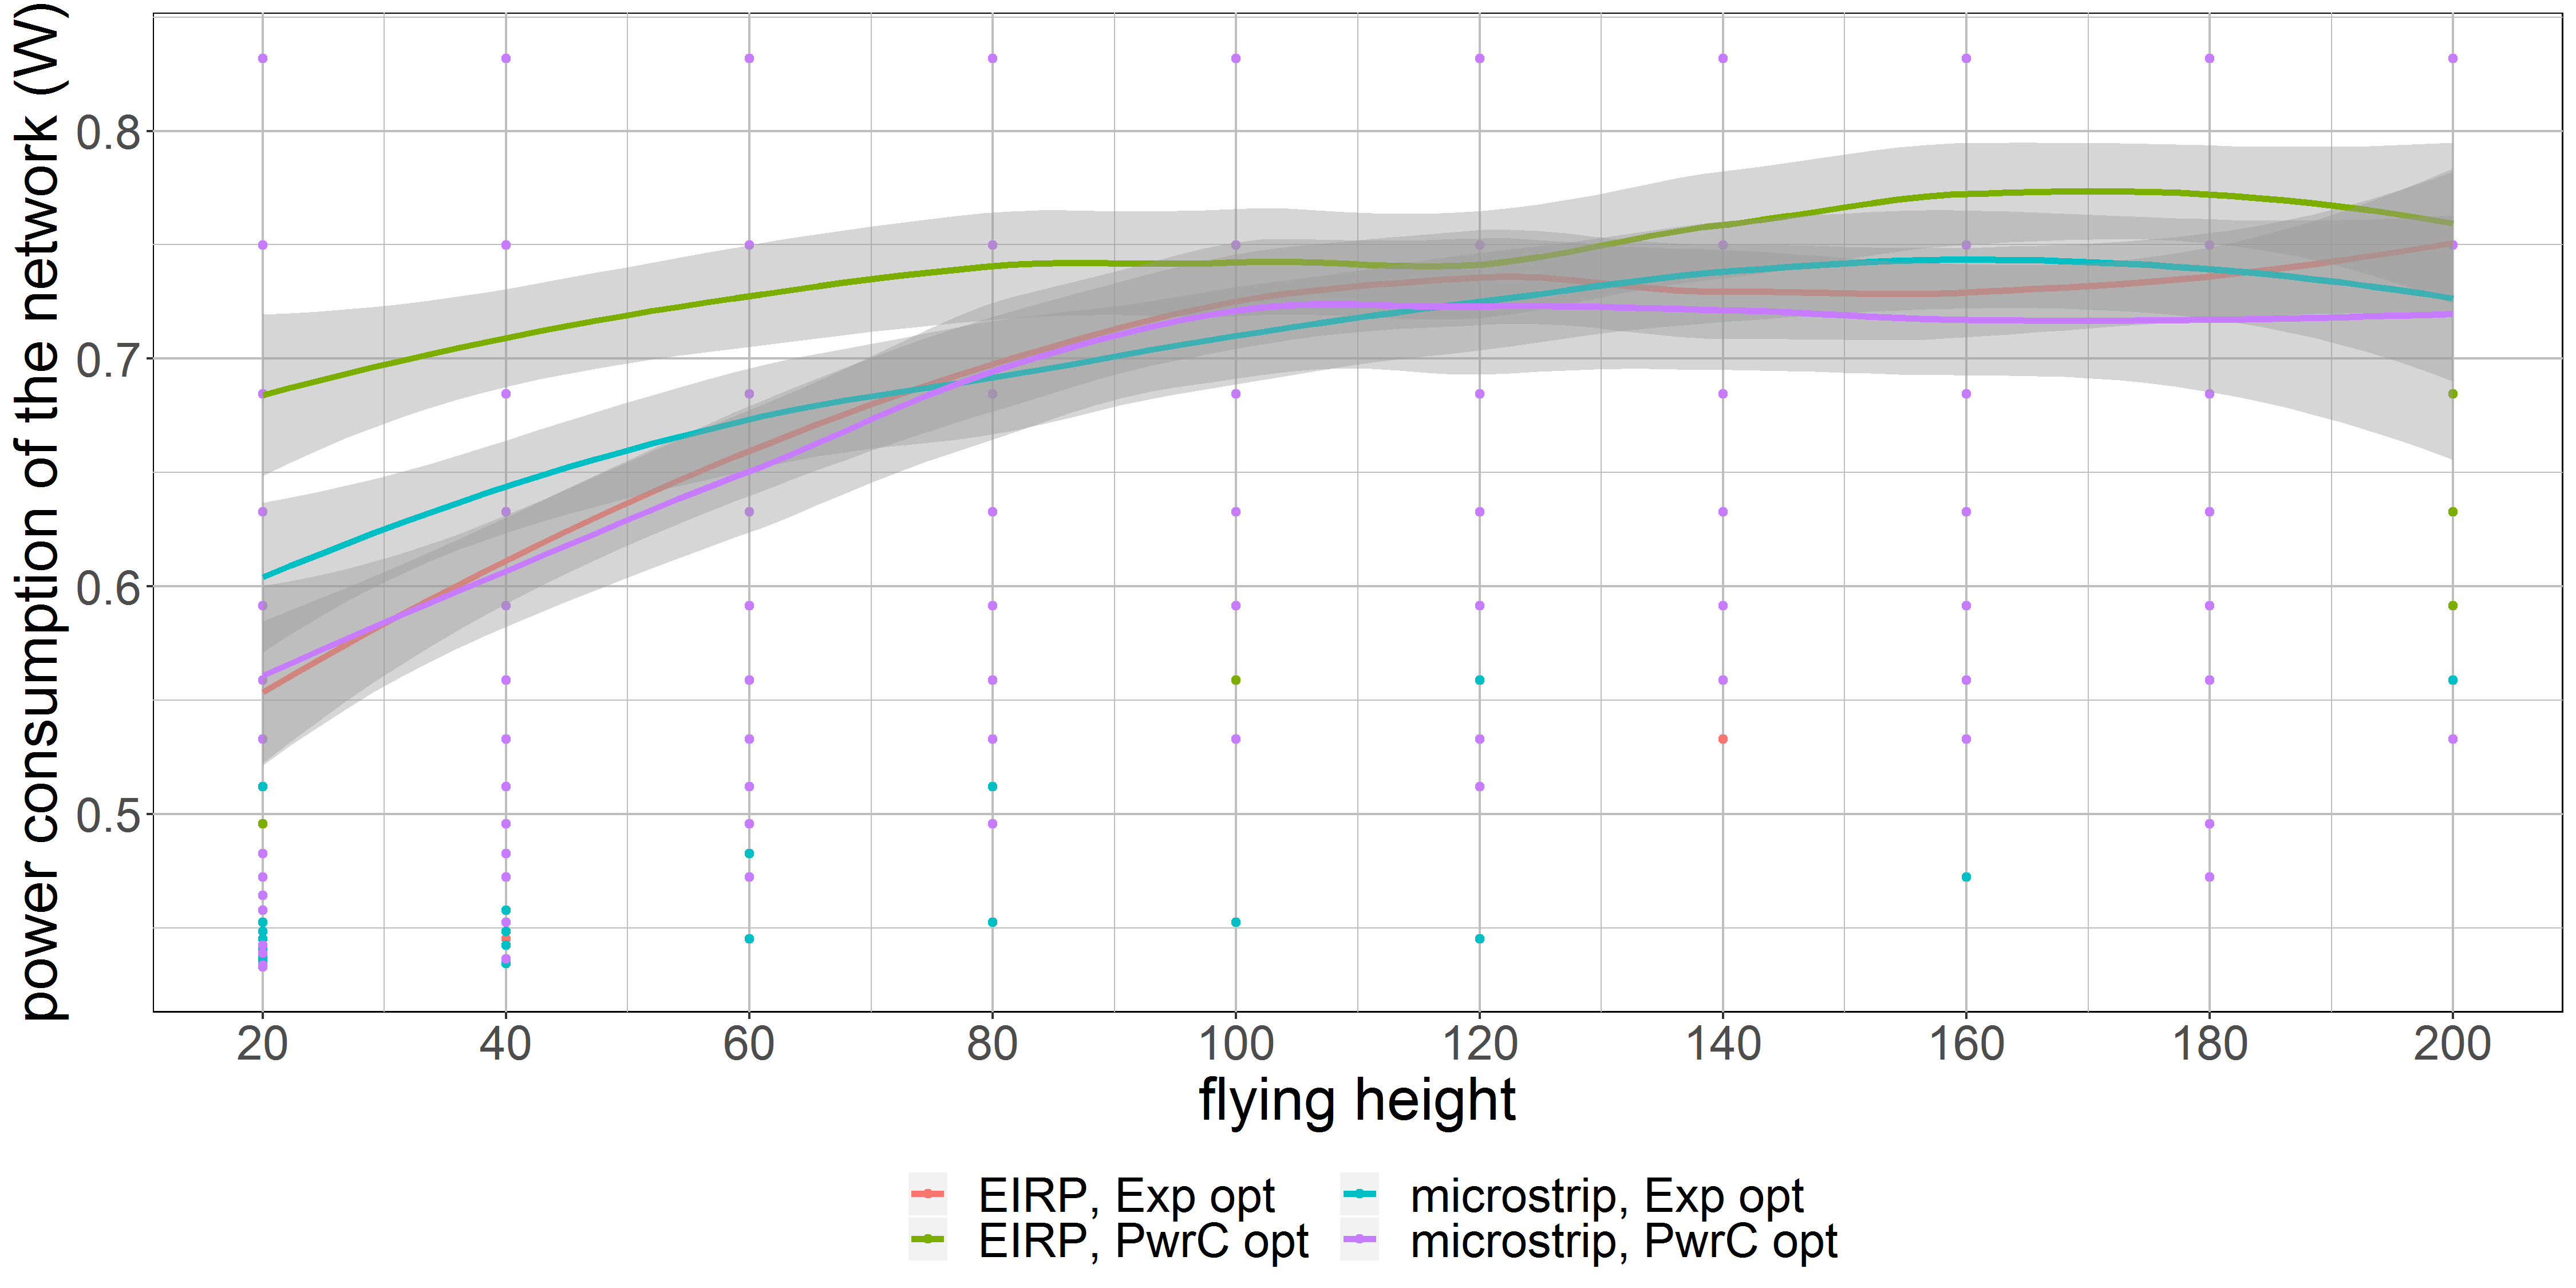
\includegraphics[width=\textwidth]{../results/s2/fhvspc.png}
  \caption{The influence of the flying height on the total power consumption of the network.}
  \label{fig:s2fhvspc}
\end{figure}
\textcolor{red}{Uitleg over deze grafiek}

Chart  \ref{fig:s2fhvscov} shows that the flying height has a positive influence on the user coverage. 
When a \gls{UABS} flies higher, there is less path loss between the user and the drone caused by buildings but also the path loss to neighbouring 
users decreases as explained 
with figure \ref{fig:prove} and \ref{fig:schematicprove}. 
Also the increasing \gls{DL} exposure  from figure \ref{fig:s2fhvsdl} confirms the that the
user coverage should grow.
As mentioned before, a power consumption optimized network will result in few high powered \gls{UABS}s. 
The tool removes all \gls{UABS}s except the one with most users. 
The network therefore exist out of one high powered \gls{UABS} compared to the exposure optimized network with one drone which 
will be less powered. Since green has a higher power level, also more users will be covered.

When replacing the fictional \gls{EIRP} antenna with a microstrip patch antenna, the percentage of covered users drops for both 
optimization strategies. This is because users who have a higher horizontal distance between themselves and the \gls{UABS}, 
experience a higher attenuation. Also, when a microstrip patch antenna is positioned higher, the range of the antenna increases 
since the angle between the user and the \gls{UABS}s main lob decreases. The user will therefore experience less attenuation.

It becomes also clear that this advantage is limited. For a scenario of 224 users and one drone, the user coverage won’t increase
 significantly any more around an altitude of 120m.

\begin{figure}[h!]
  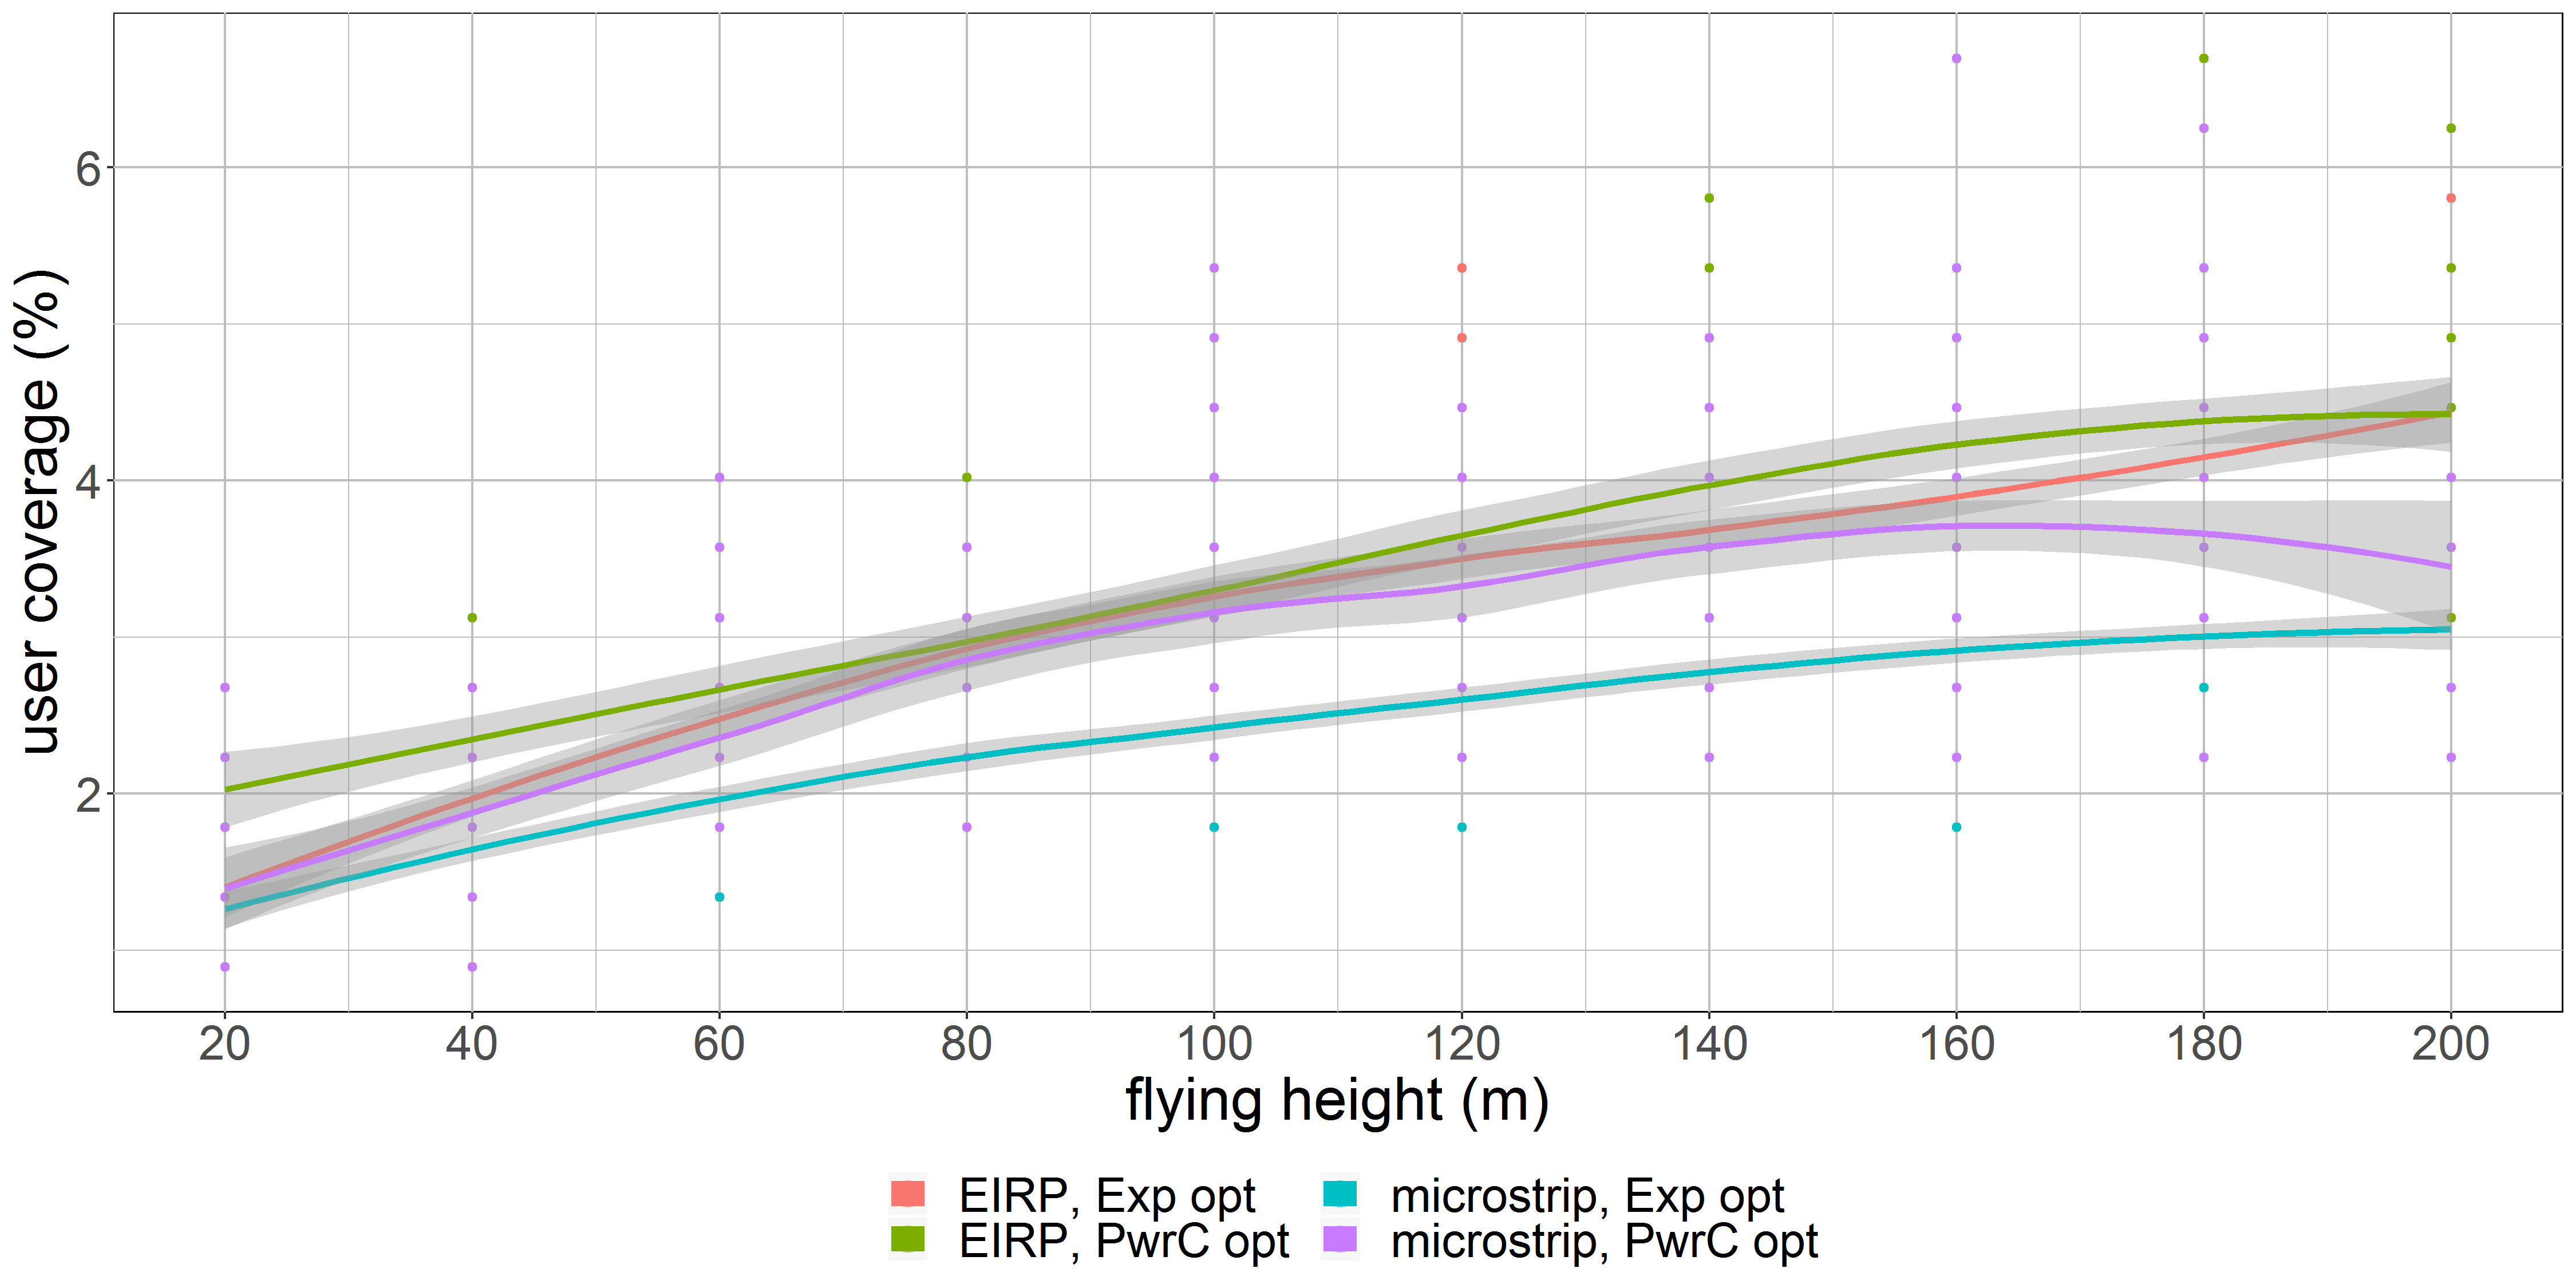
\includegraphics[width=\textwidth]{../results/s2/fhvscov.png}
  \caption{This graph shows the percentage of covered users by one drone for different flying heights.}
  \label{fig:s2fhvscov}
\end{figure}

Chart \ref{fig:s2fhvssar} shows the whole body SAR10g, deducted from all electromagnetic sources. This being exposure of all \gls{UABS}s,
 the uplink exposure from the user’s own device and the exposure of the devices from all other users. 
 Thereafter, the weighted average of all whole body SAR10g values in the network is calculated with the 50th and 95th percentile 
 being the most important values. This is because not only the mean values are important but also users who experience higher 
 levels of whole body SAR10g.


\begin{figure}[h!]
  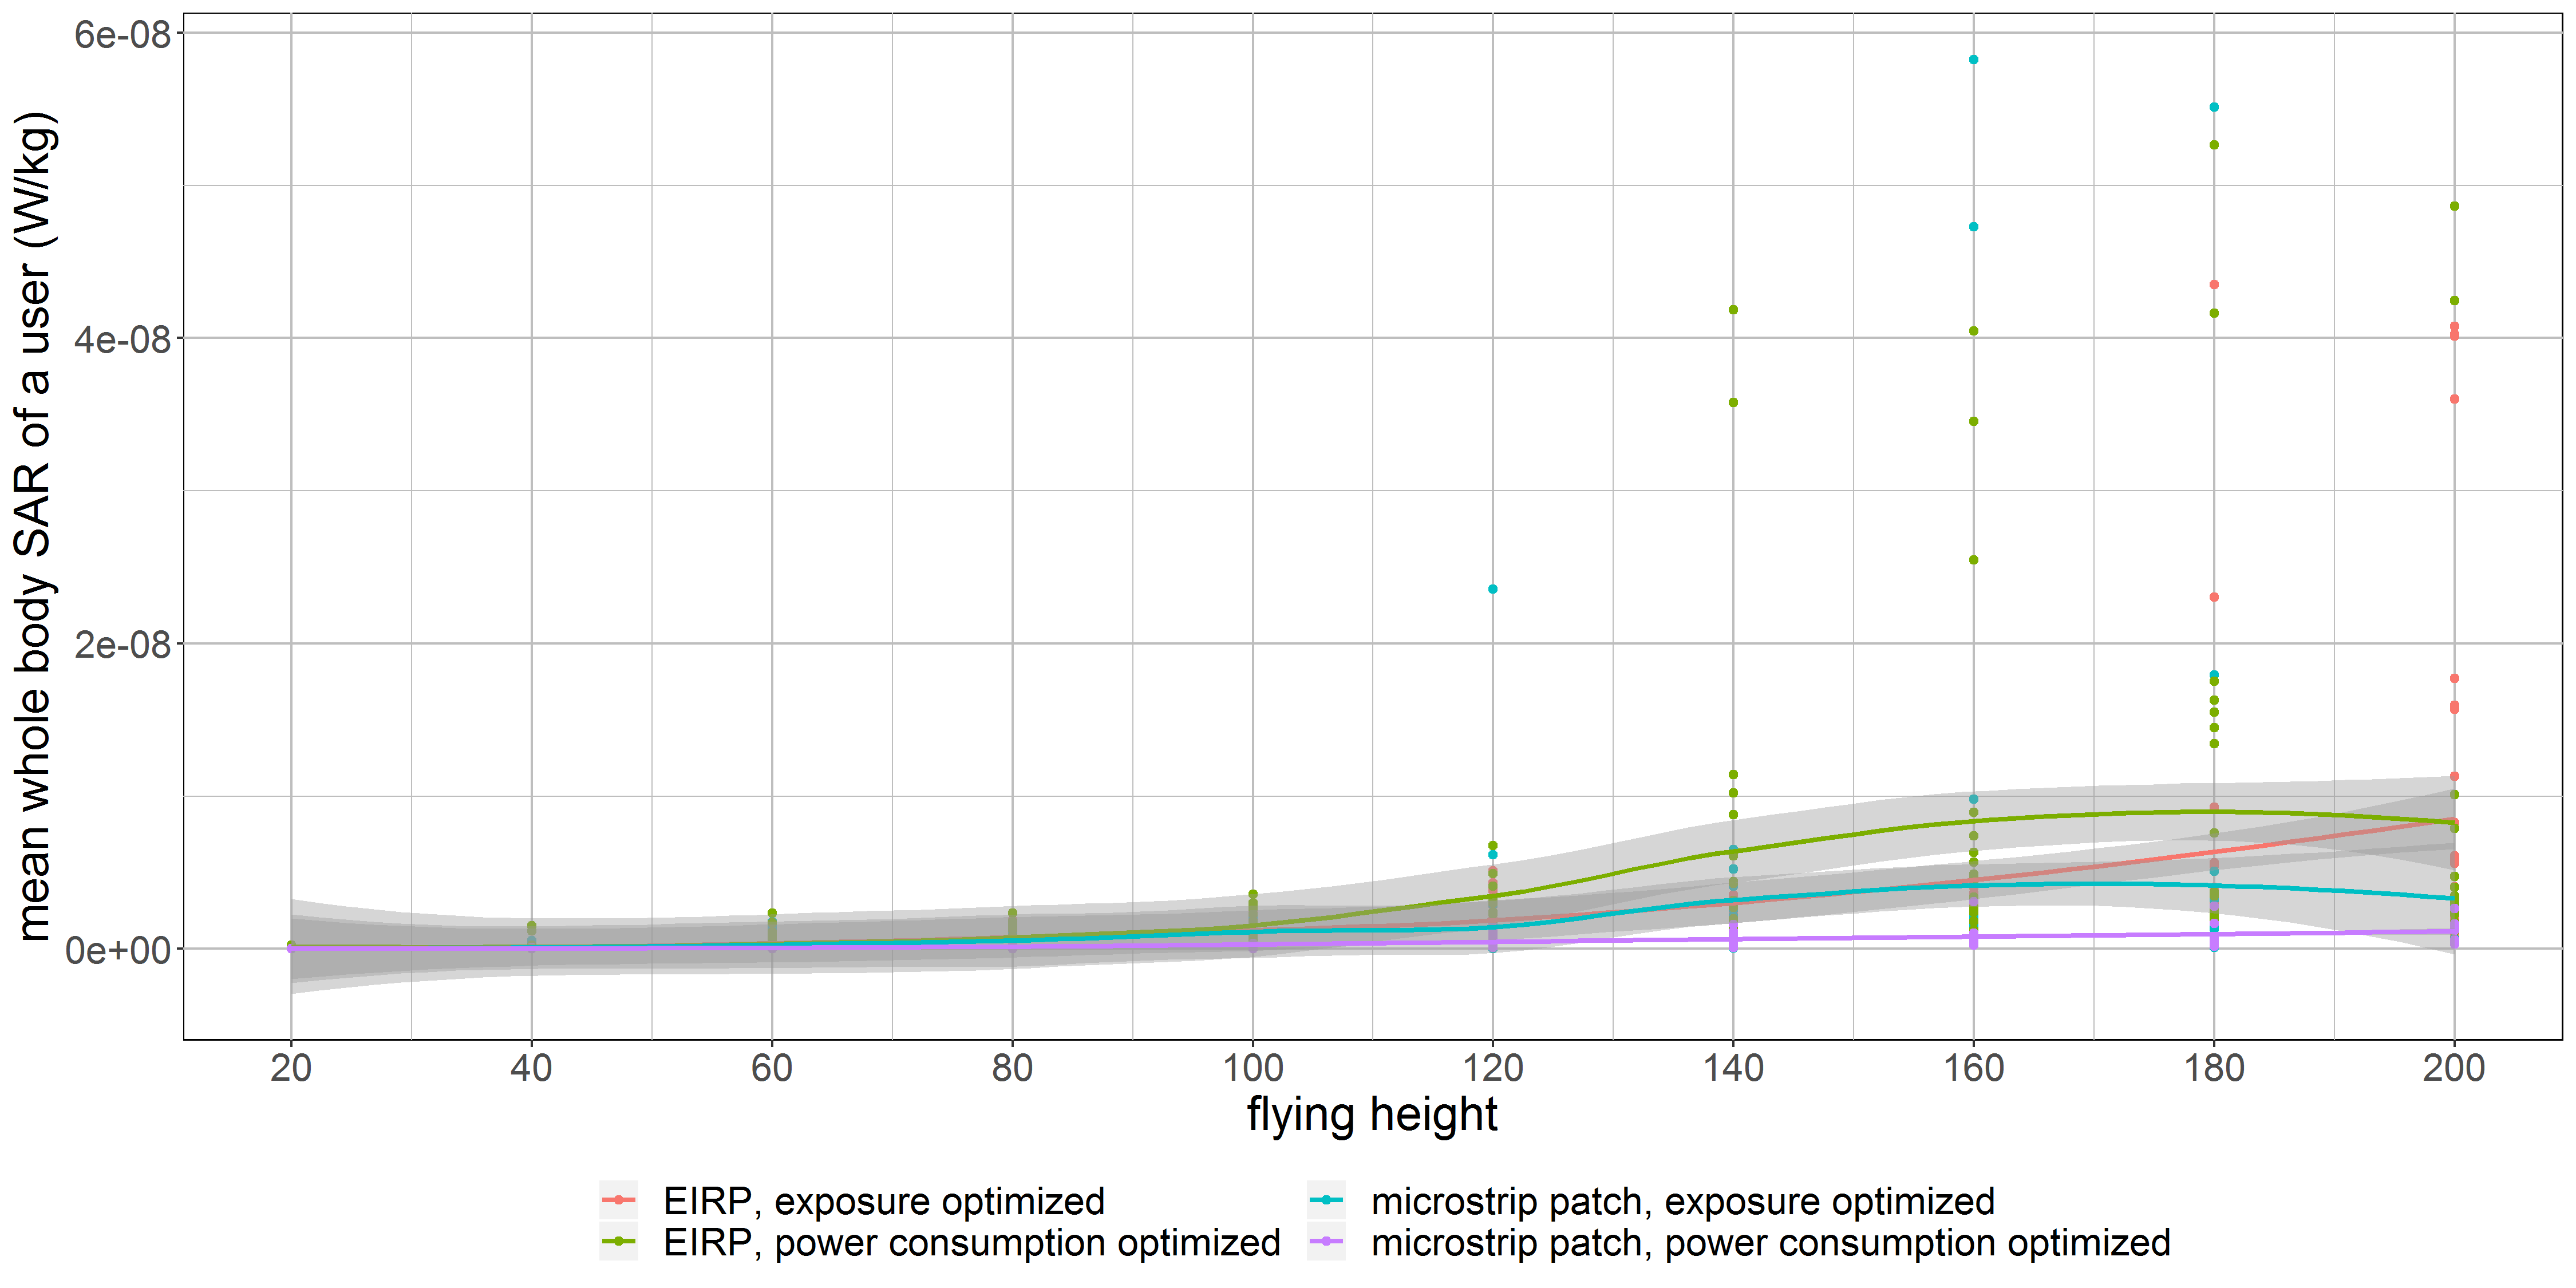
\includegraphics[width=\textwidth]{../results/s2/fhvssar.png}
  \caption{The influence of the flying height on the weighted average $SAR_{10g}$ of users in the network.}
  \label{fig:s2fhvssar}
\end{figure}

When investigating the 3 different sources for the total \gls{SAR}-values from \ref{fig:s2fhvssar}, we see 
that the radiation from all different \gls{UABS}s is the main factor followed by the near field radiation from the user's own device.
The far field radiation from other \gls{UE} has barely influence. It looks like it is zero but it is just very low compared to the other two values. 
\begin{figure}[h!]
  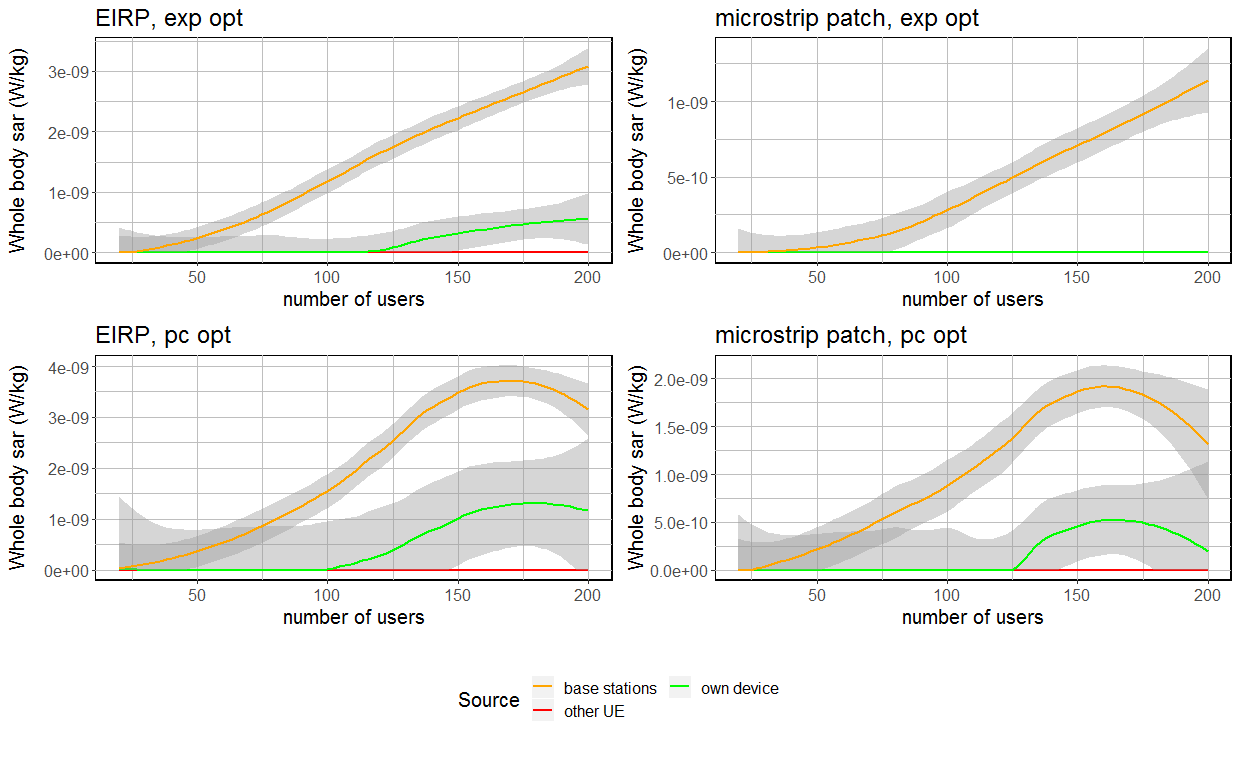
\includegraphics[width=\textwidth]{../results/s2/fhSARMatrix.png}
  \caption{This figure shows how different sources are influenced by an increasing flying height.}
  \label{fig:s2shfourSourcesMatrix}
\end{figure}

\FloatBarrier
\subsection{Influence of the number of users}

The number of covered users increase linearly compared to the number of users present in the network.
An \gls{isotropicradiator} has no attenuation and is therefore able to reach more users. On the other side, an power consumption 
optimized network with only one drone will result in a high powered \gls{UABS} as explained before and is therefore also able to 
cover more users. The complete opposite is a microstrip patch in an exposure optimized network (which is the blue line in figure \ref{fig:s2uvsnumcovusers})
and covers the least number of users.

\begin{figure}[h!]
  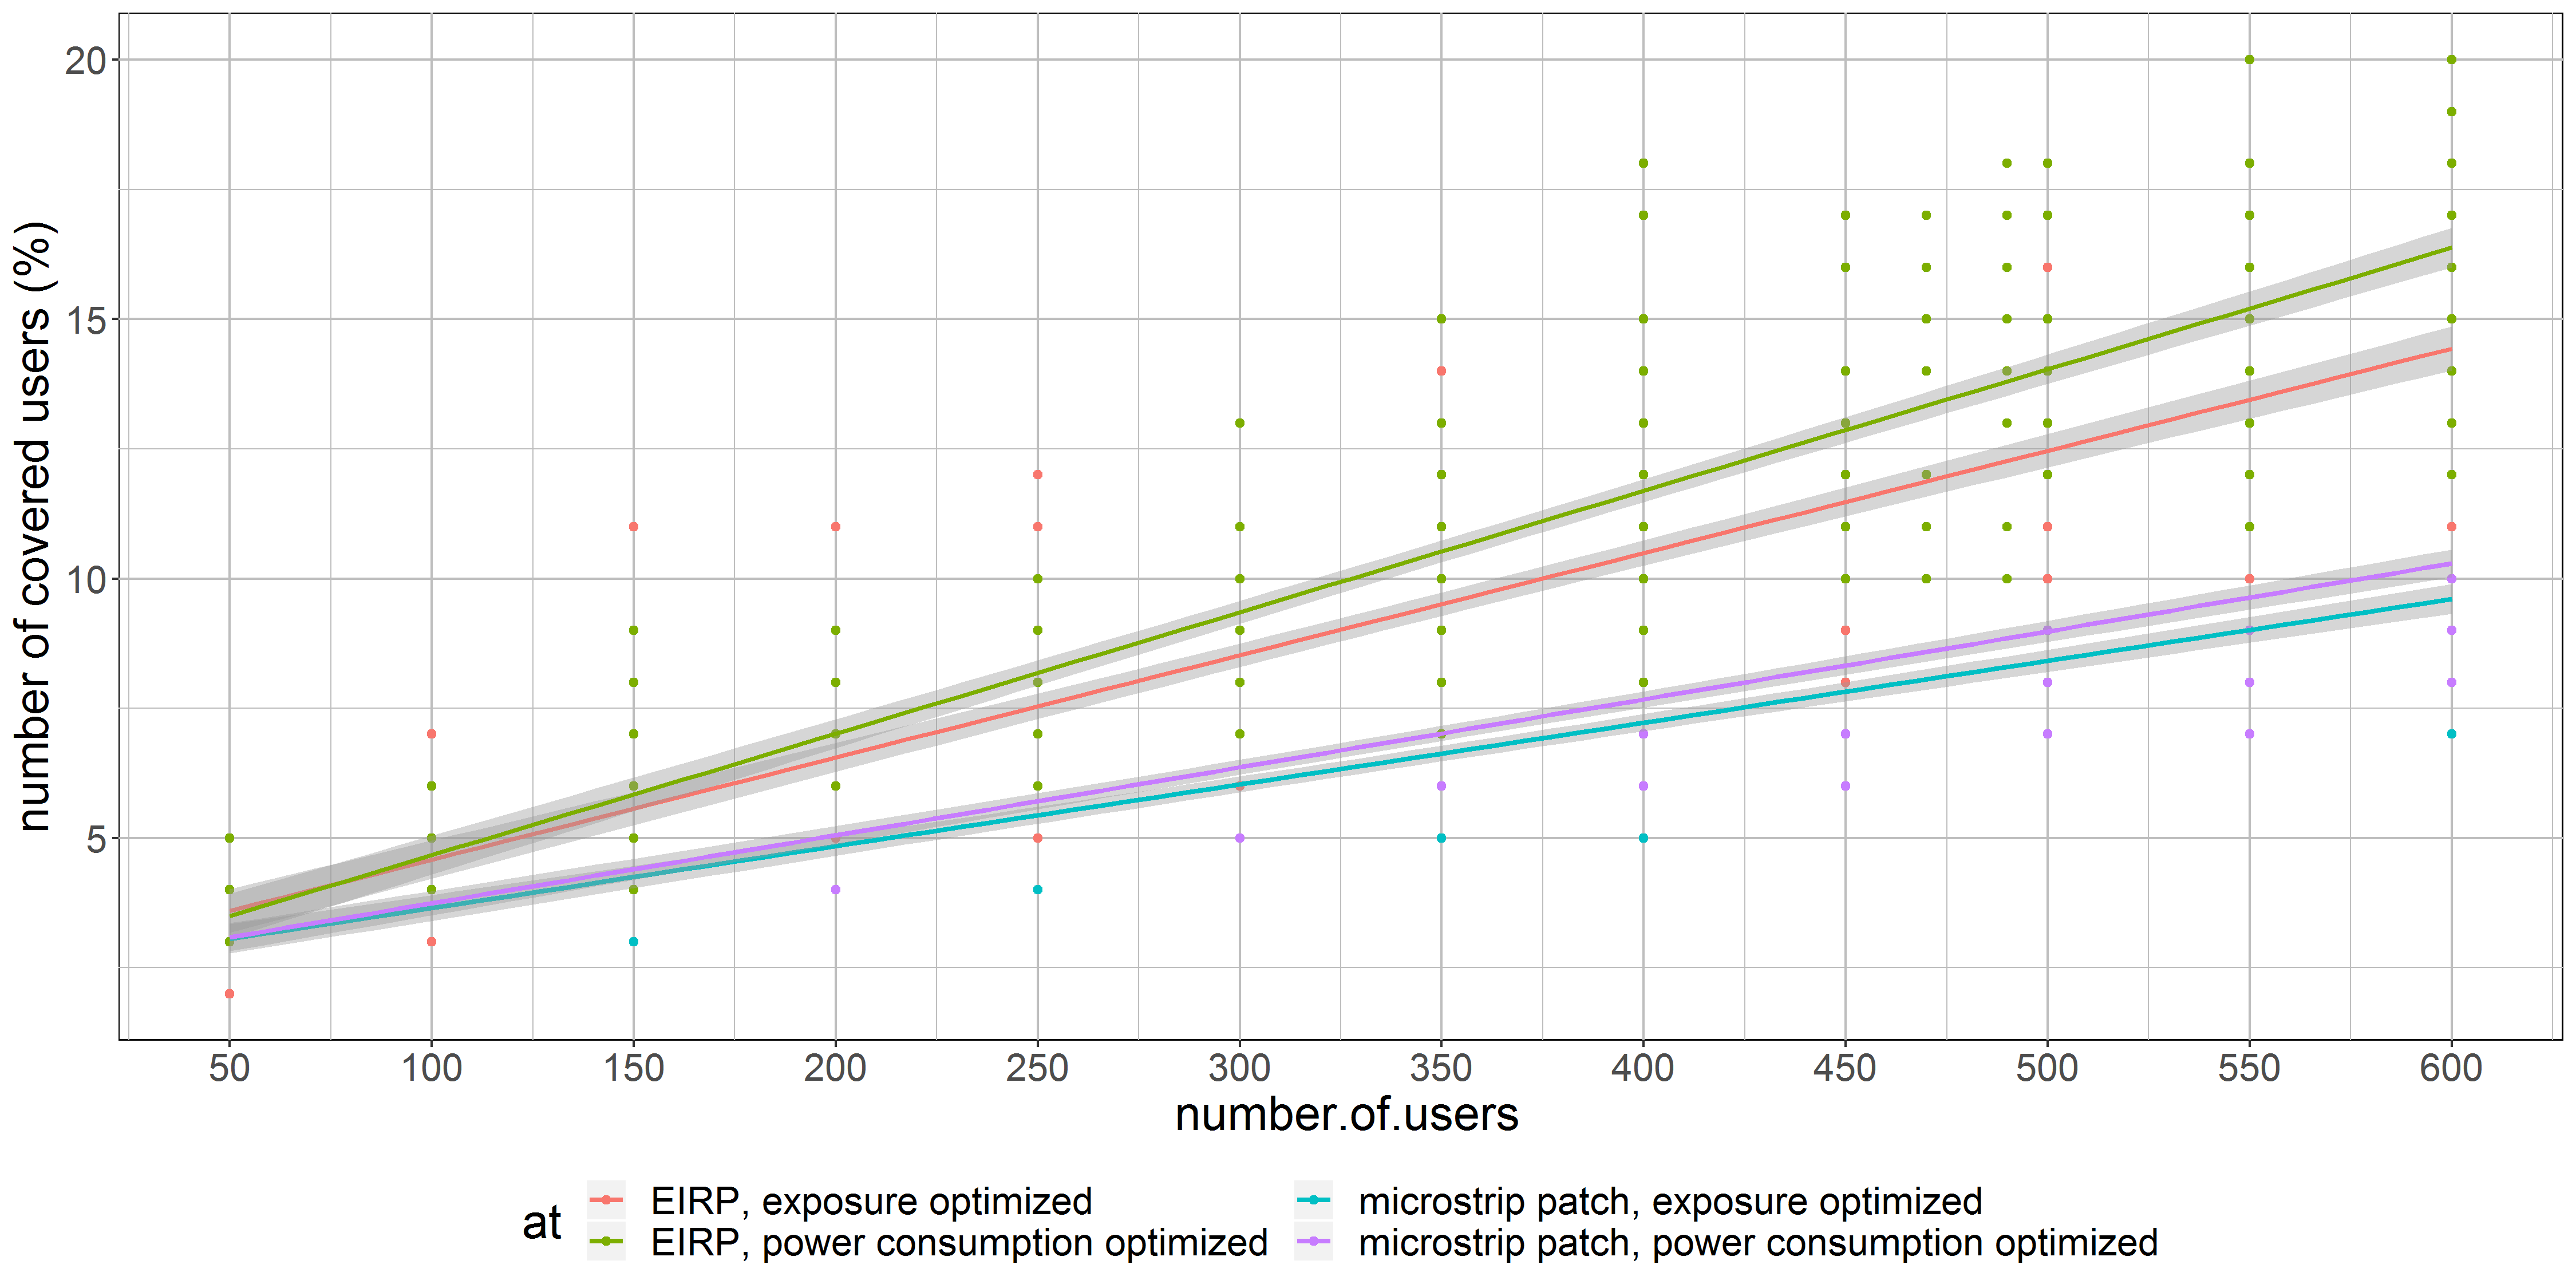
\includegraphics[width=\textwidth]{../results/s2/uvsnumcovusers.png}
  \caption{The influence of increasing traffic on user coverage.}
  \label{fig:s2uvsnumcovusers}
\end{figure}

The linear regression lines from \ref{fig:s2uvsnumcovusers} can be predicted with the equations in \ref{eq:numcovusers}.

\begin{equation}
\text{number of users =}
    \begin{cases}
      y = 0,0233x + 2,3553 & \text{if EIRP and pc}\\
      y = 0,0197x + 2,6144  & \text{if EIRP and exp}\\
      y = 0,0131x + 2,4371  & \text{if micro and pc}\\
      y = 0,0119x + 2,4652  & \text{if micro and exp}
    \end{cases} 
    \label{eq:numcovusers}      
\end{equation}

The percentage of covered users is achieved by taking the equations from \ref{eq:numcovusers} and dividing them by $x$.
Figure \ref{fig:s2uvscov} shows a decreasing logarithmic behaviour because the regression lines from  \ref{fig:s2uvsnumcovusers} have a slope of less then 0.5.
So in other words, the  percentage of covered users for a sparsely populated network is more compared to the percentage of users in high dense populations.

\begin{figure}[h!]
  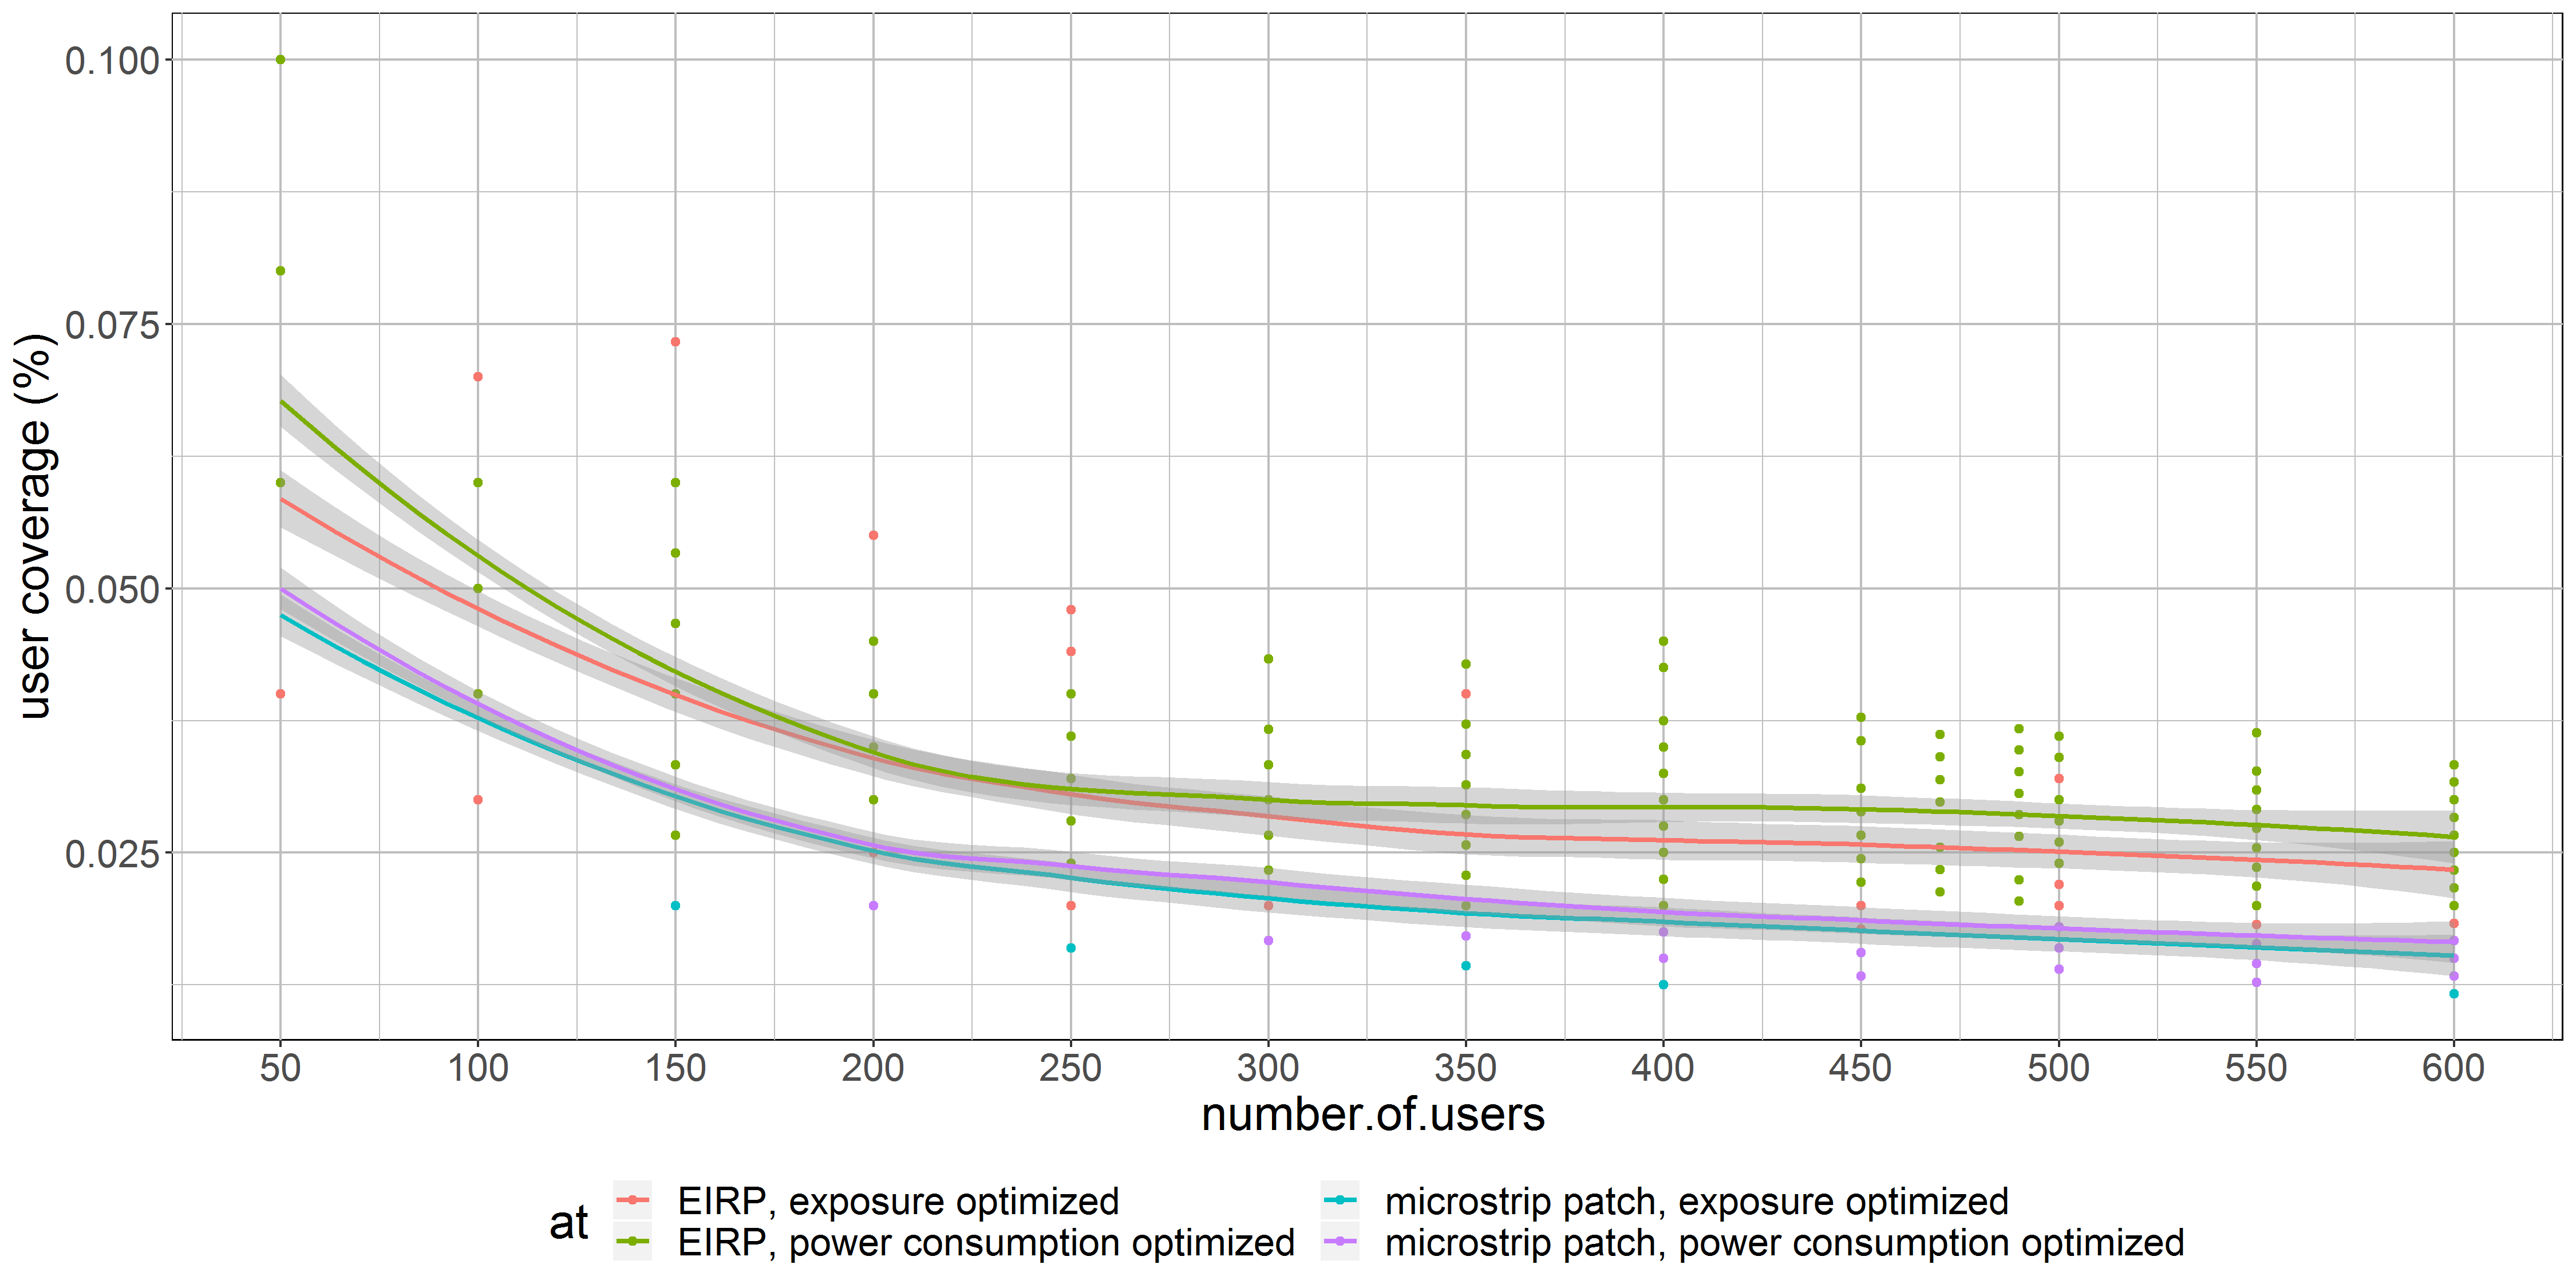
\includegraphics[width=\textwidth]{../results/s2/uvscov.png}
  \caption{The influence of increasing traffic on user coverage.}
  \label{fig:s2uvscov}
\end{figure}

The downlink exposure is directly influenced by the number of covered users (figure \ref{fig:s2uvsdl}). 
The electromagnetic exposure increases when more users are covered and since an \gls{isotropicradiator} in a power consumption optimized network (green)
will have the highest coverage, also the \gls{DL} electromagnetic radiation from \gls{UABS}s will be higher.

\begin{figure}[h!]
  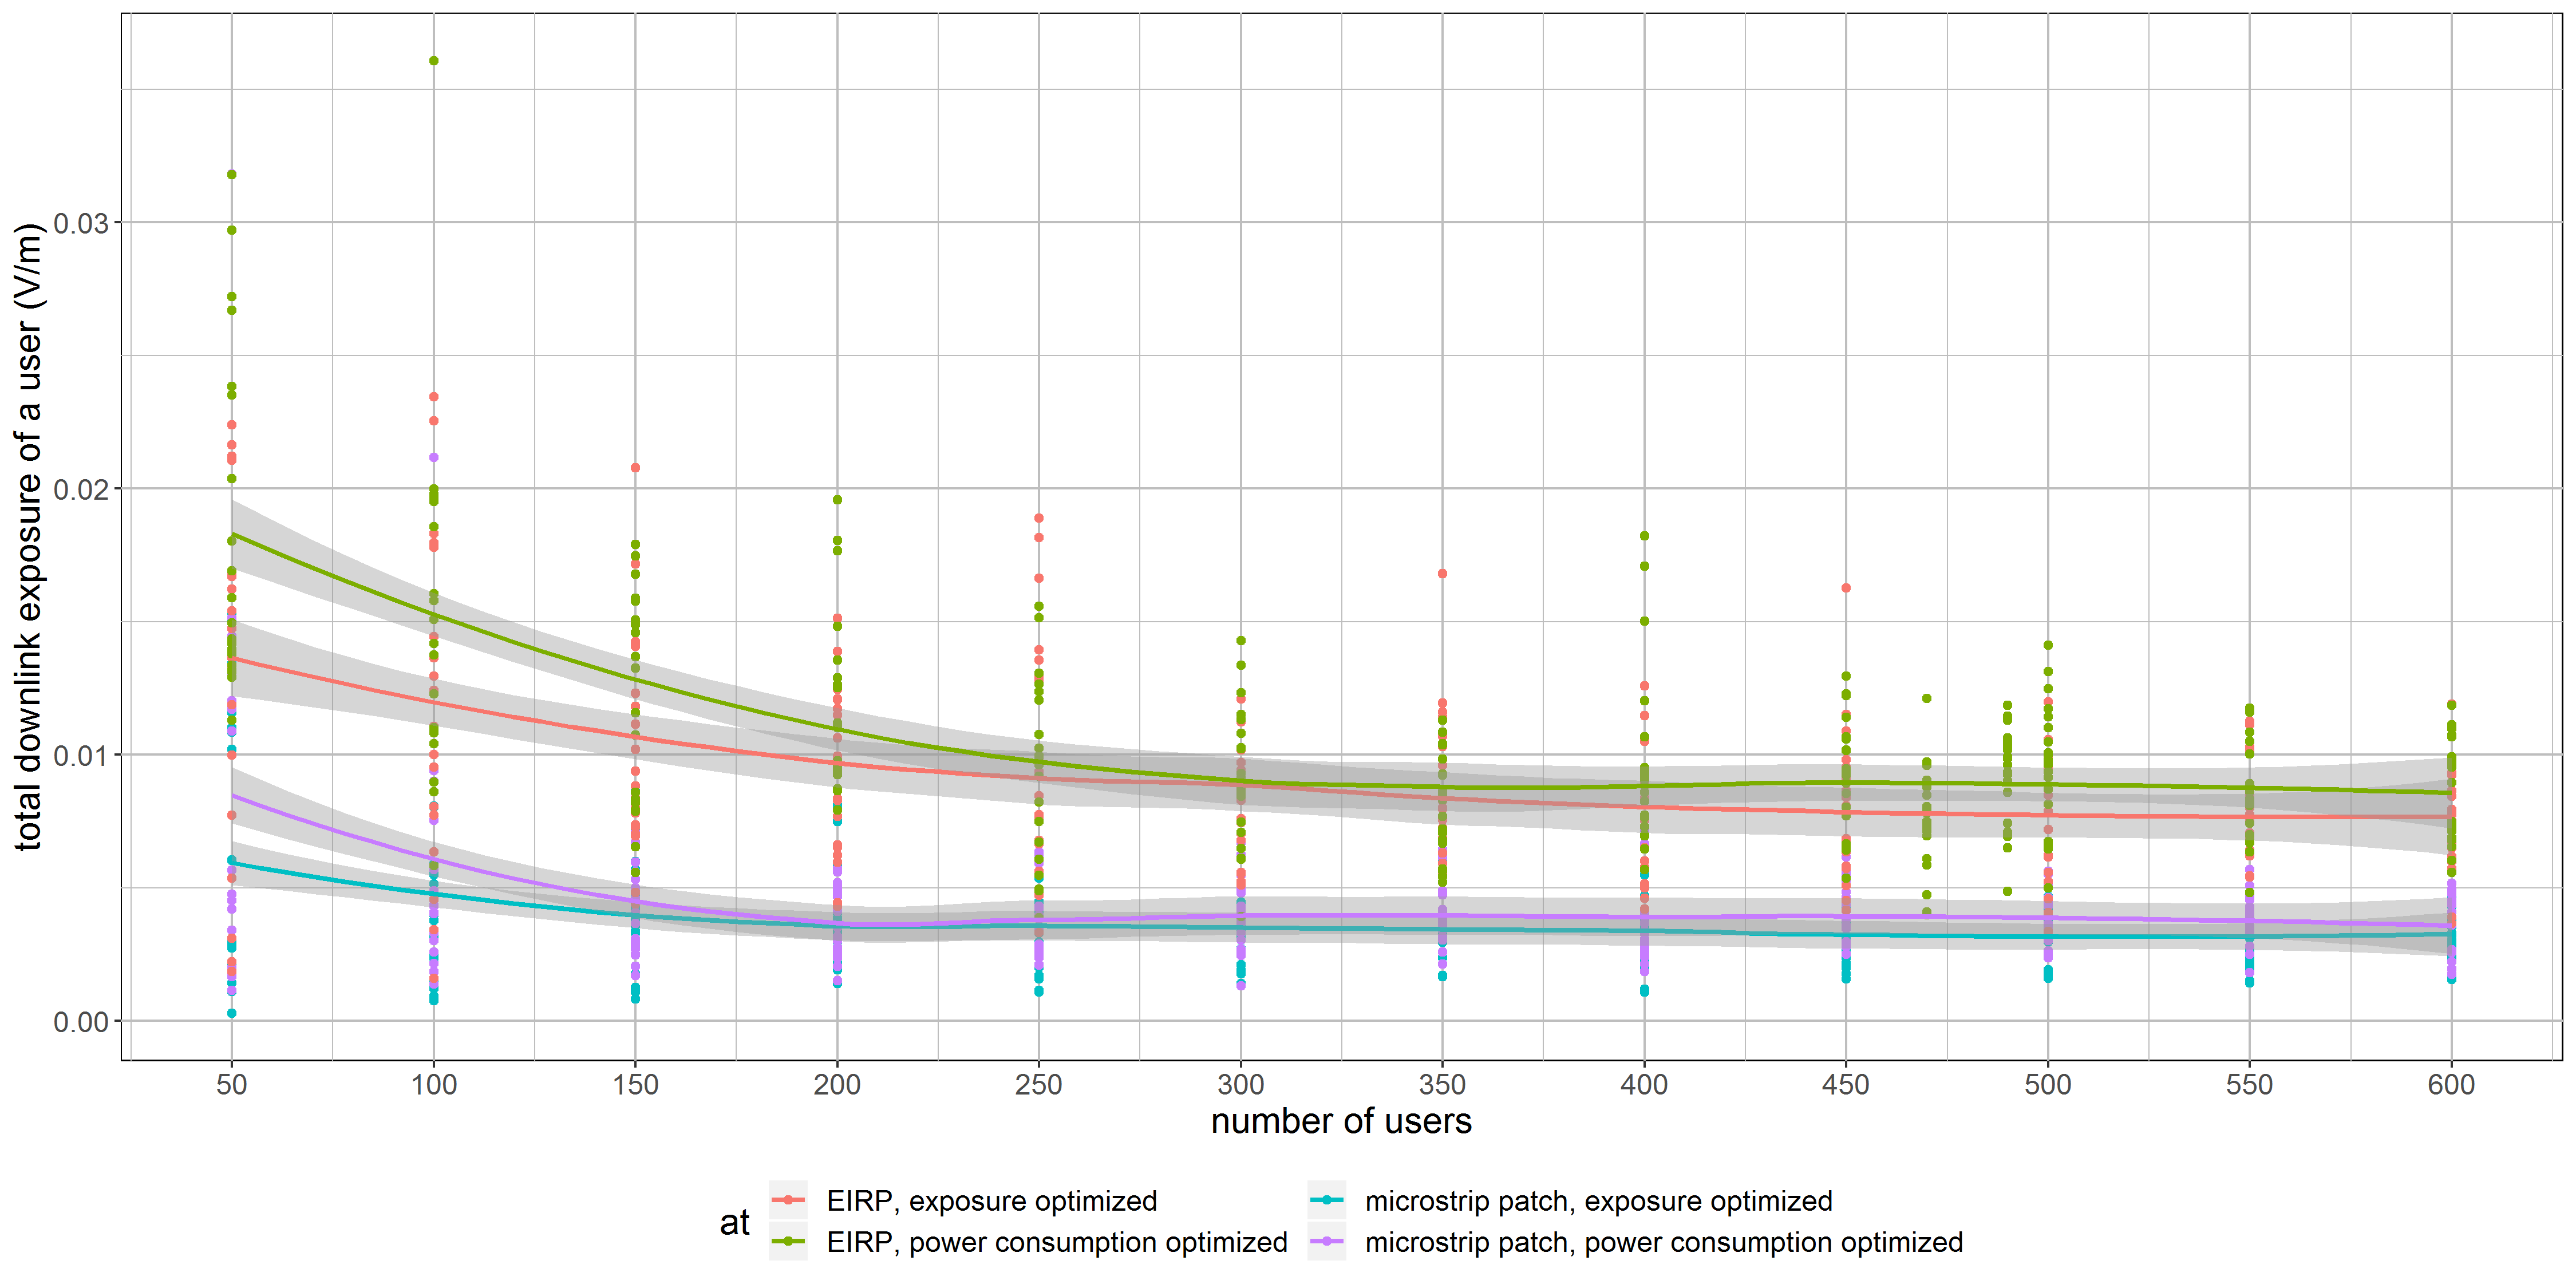
\includegraphics[width=\textwidth]{../results/s2/uvsdl.png}
  \caption{The influence of increasing traffic on downlink exposure.}
  \label{fig:s2uvsdl}
\end{figure}

\begin{figure}[h!]
  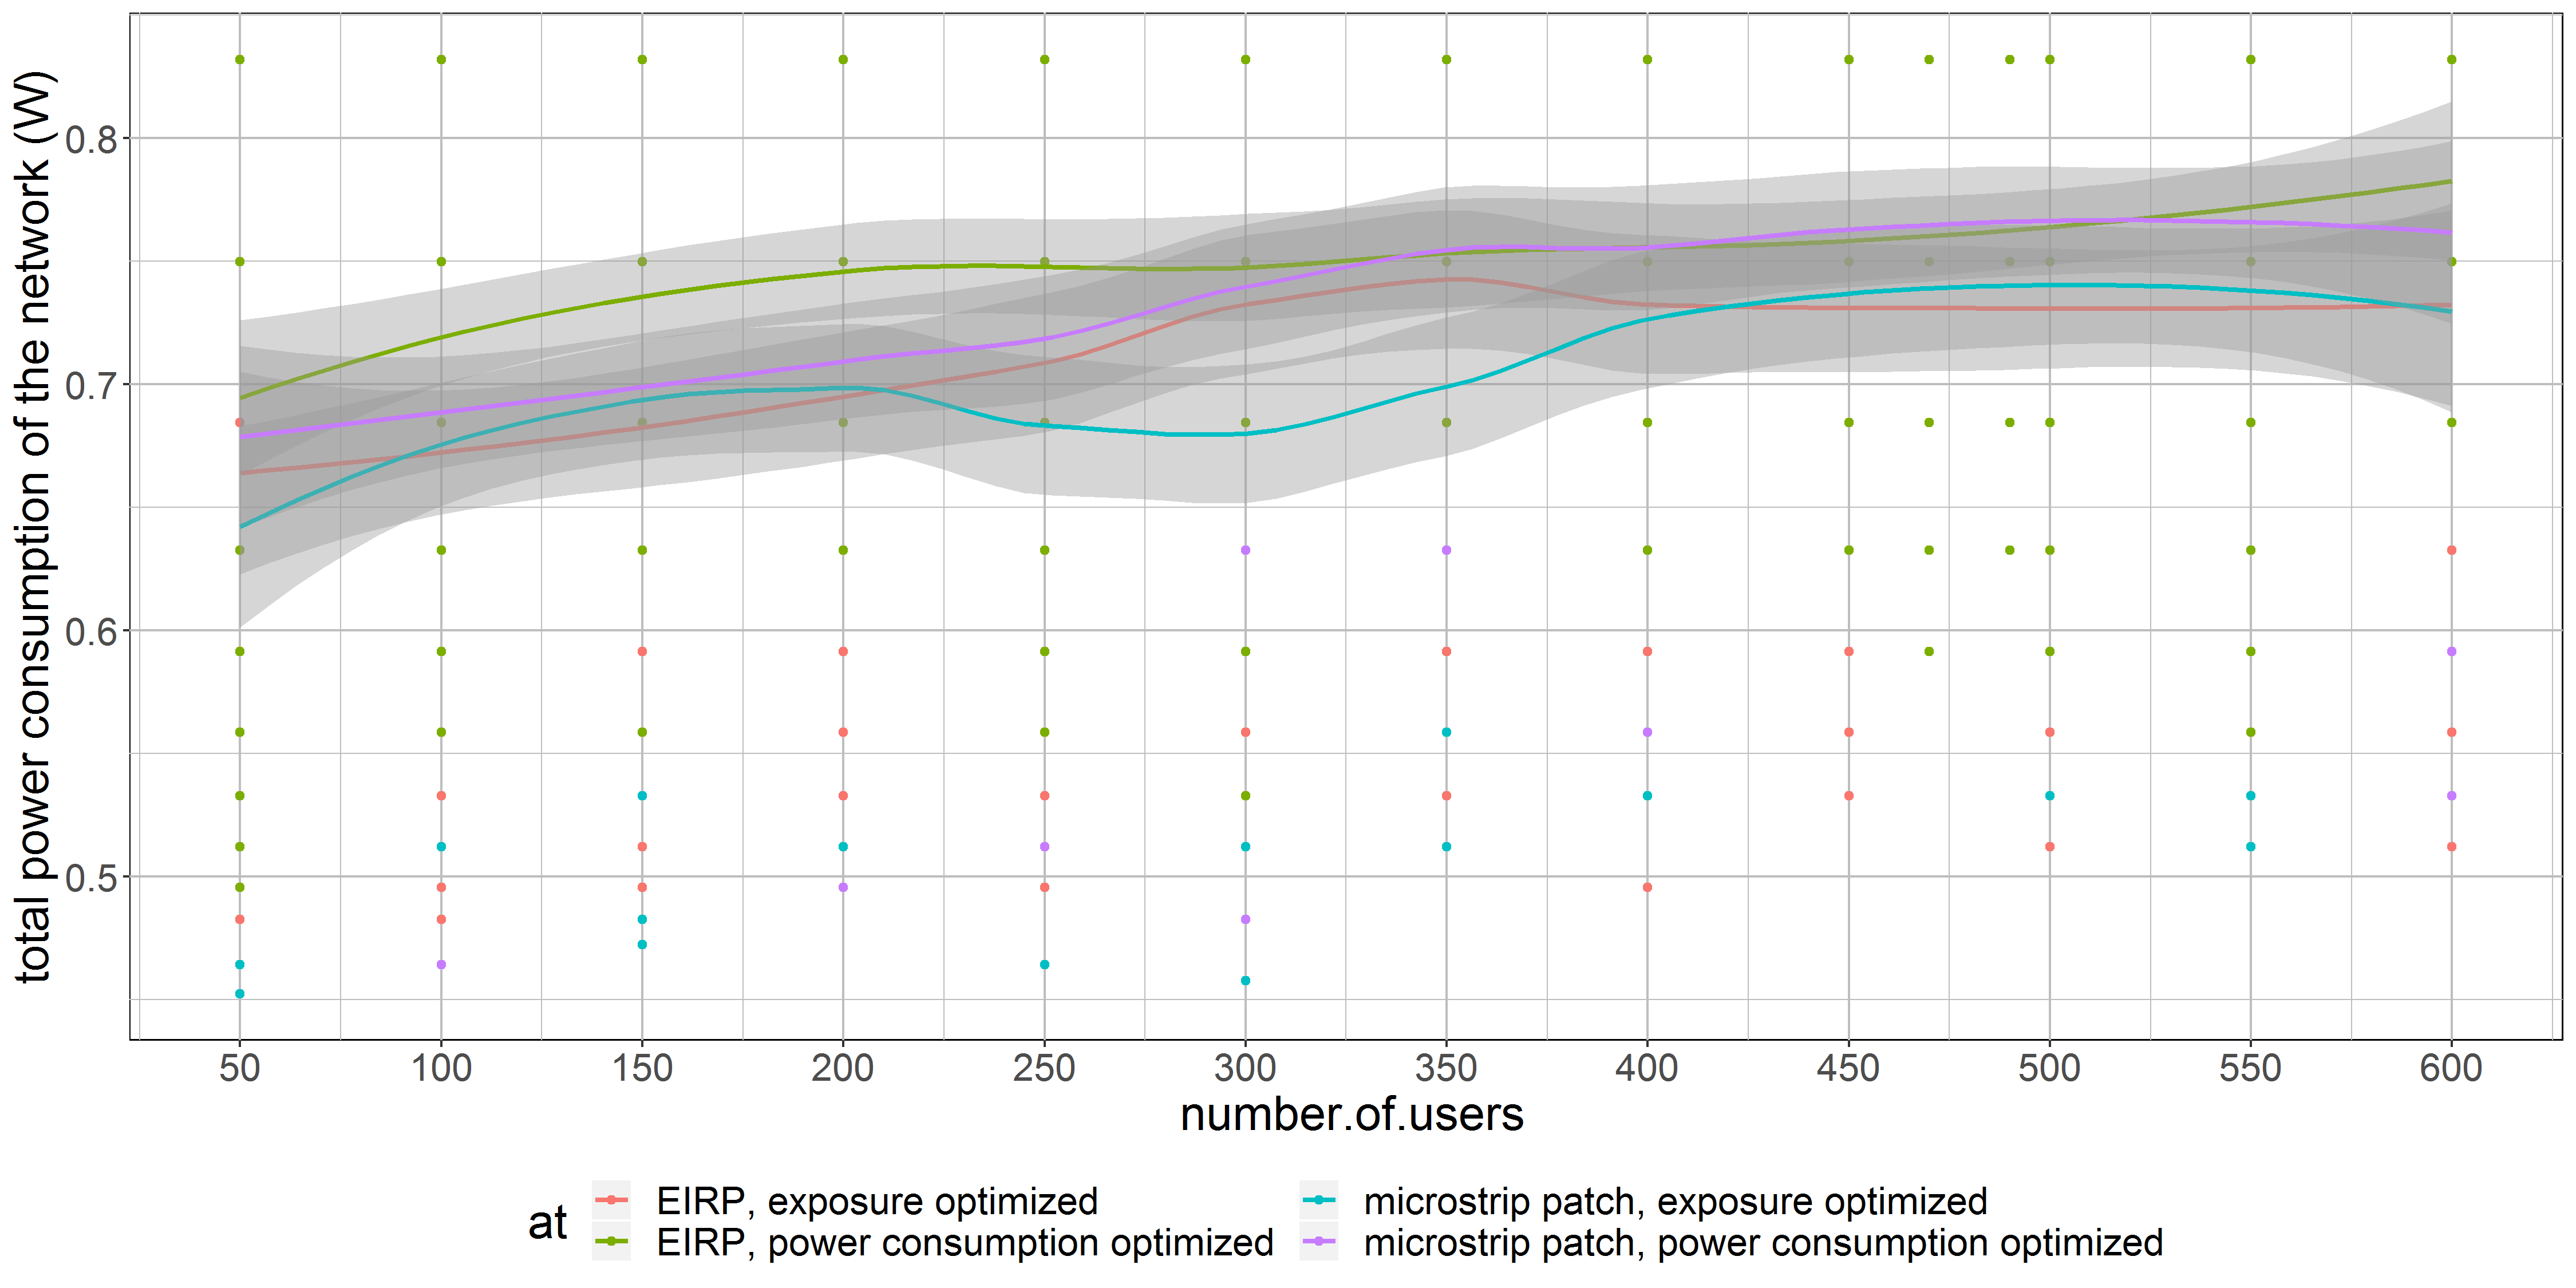
\includegraphics[width=\textwidth]{../results/s2/uvspc.png}
  \caption{The influence of increasing traffic on the total power consumption.}
  \label{fig:s2uvspc}
\end{figure}

The optimization strategies only consider \gls{DL} exposure and power consumption.
However, how much radiation is absorbed by the users originating from all sources is shown in \ref{s2uvssar} and the relative position of 
the four configurations do not differ compared to the \ref{s2uvssar}. So an \gls{DL} exposure optimized network with an \gls{isotropicradiator}
 which result in the highest electromagnetic exposure for this scenario will also have the highest specific absorption rate according to figure
 \ref{fig:s2uvssar}. The same applies for the other configurations as well.

\begin{figure}[h!]
  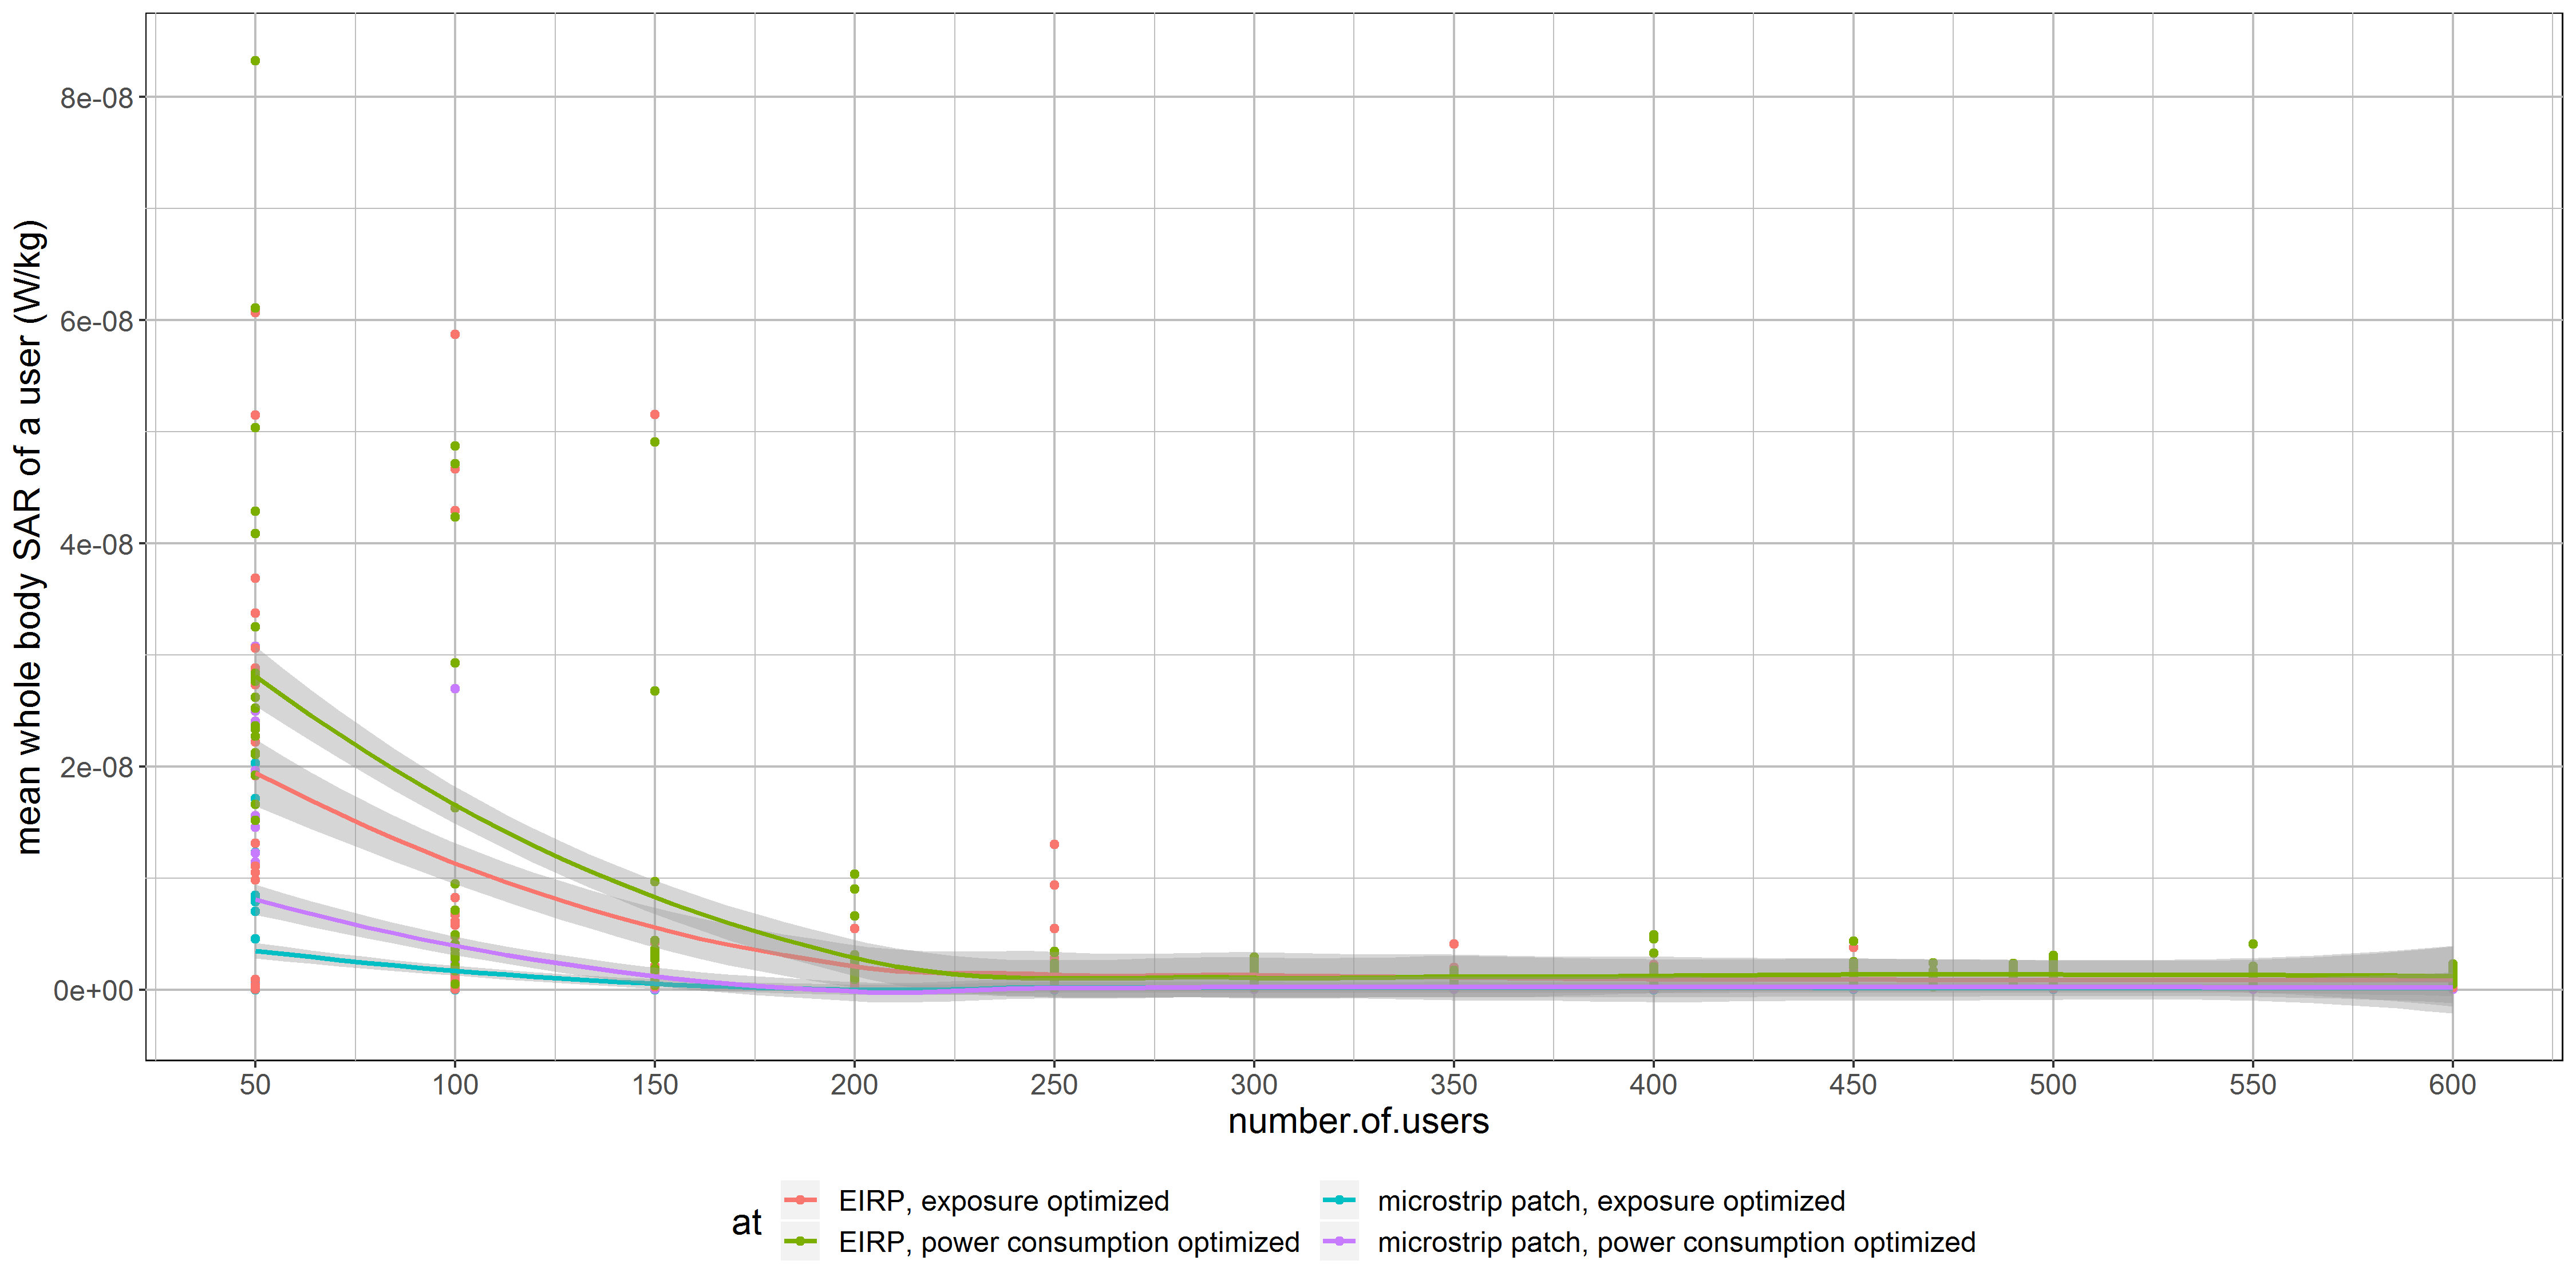
\includegraphics[width=\textwidth]{../results/s2/uvssar.png}
  \caption{This figure shows how different sources are influenced by an increasing number of users. }
  \label{fig:s2uvssar}
\end{figure}

Figure \ref{fig:s2fourSourcesMatrix} investigates the assets of each source to the \gls{SAR}. All four 
configuration show that for 200 users and up, base stations are the main source of electromagnetic radiation.

For less users, the electromagnetic radiation from the user's device is much higher. Chart \ref{fig:s2uvscov} already 
showed that for 200 users and less, the number of covered user's is higher  but there is still only one \gls{UABS} available.
So \gls{UE}  need to radiate much more in order to still be able to reach that one drone.

The red line proves that the far field electromagnetic exposure from other users their device can be neglected. The \gls{SAR} from 
neighbouring devices is not zero as it looks from figure \ref{fig:s2fourSourcesMatrix} but is just really low compared to the much higher
\gls{SAR}-values from other sources.

\begin{figure}[h!]
  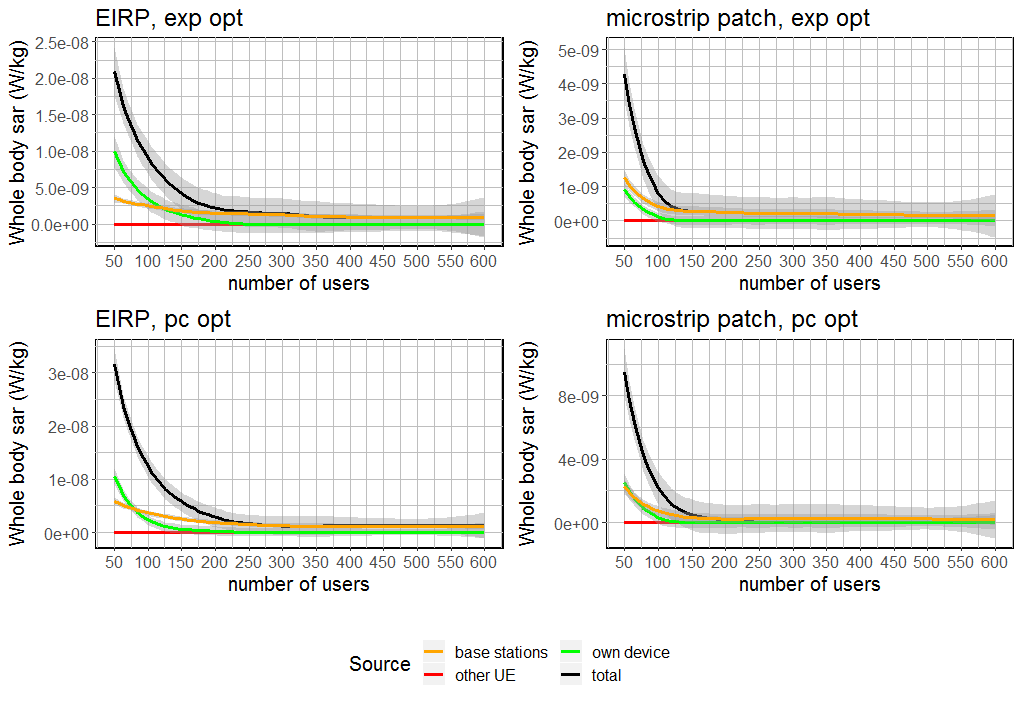
\includegraphics[width=\textwidth]{../results/s2/fourSourcesMatrix.png}
  \caption{This figure shows how different sources are influenced by an increasing number of users. }
  \label{fig:s2fourSourcesMatrix}
\end{figure}

%%%%%%%%%%%%%%%%%%%%%%%%%%%%%%%%%%%%%%%%%%%%%%%%%%%%%%%%%%%%%%%%%%%%%%%%%%%%%%%%%%%%%%%%%%%%%%%%%%%%%%%%%%%%%s
\section{Scenario 3: Unlimited Drones}
\subsection{Influence of the flying altitude}

This scenario examines the same cases as scenario 2 but there is no restriction on the number of \gls{UABS}s. 
Unlike in scenario 2, fig. \ref{fig:s3fhvsdl} and \ref{fig:s3fhvspc} show a clearer view on how the decision algorithms
works. Antennae in an exposure optimized network cause less downlink exposure (fig. \ref{fig:s3fhvsdl}). On the other hand, 
a network generated for optimal power consumption requires indeed less energy as proven in figure \ref{fig:s3fhvspc}. 

Figure \ref{fig:s3fhvsdl} shows how an \gls{isotropicradiator} in and power consumption optimized network has the highest exposure when 
the \gls{UABS}  is close to the ground. An power consumption optimized network results in less number of drones which can also be seen 
on figure \ref{fig:s3:fhvsnumdrones}. The network is still trying to cover as much users as possible as visible on figure 
\ref{fig:s3fhvscov} (with in this case less resources). Low flying drones need to account for increased path loss by obstructing buildings.
When the flying altitude increases, there is less path loss and the electromagnetic exposure stabilizes. The same is applicable when replacing
the \gls{isotropicradiator} with a microstrip patch antenna but users will experience less electromagnetic radiation 
because of antenna aperture. Because the algorithm still tries to cover as much users as possible, the tool will react to this by 
introducing more drones (fig \ref{fig:s3fhvsnumdrones}).

When changing the optimization strategy towards an exposure optimized network, the lowest possible electromagnetic radiation is recorded
with low flying drones at 20 m height with microstrip patch antennae. Using an \gls{isotropicradiator} automatically increases electromagnetic 
radiation because of the absence of attenuation. This behaviour results in an higher necessity of antenna carriers \ref{fig:s3fhvsnumdrones}.


\begin{figure}[h!]
  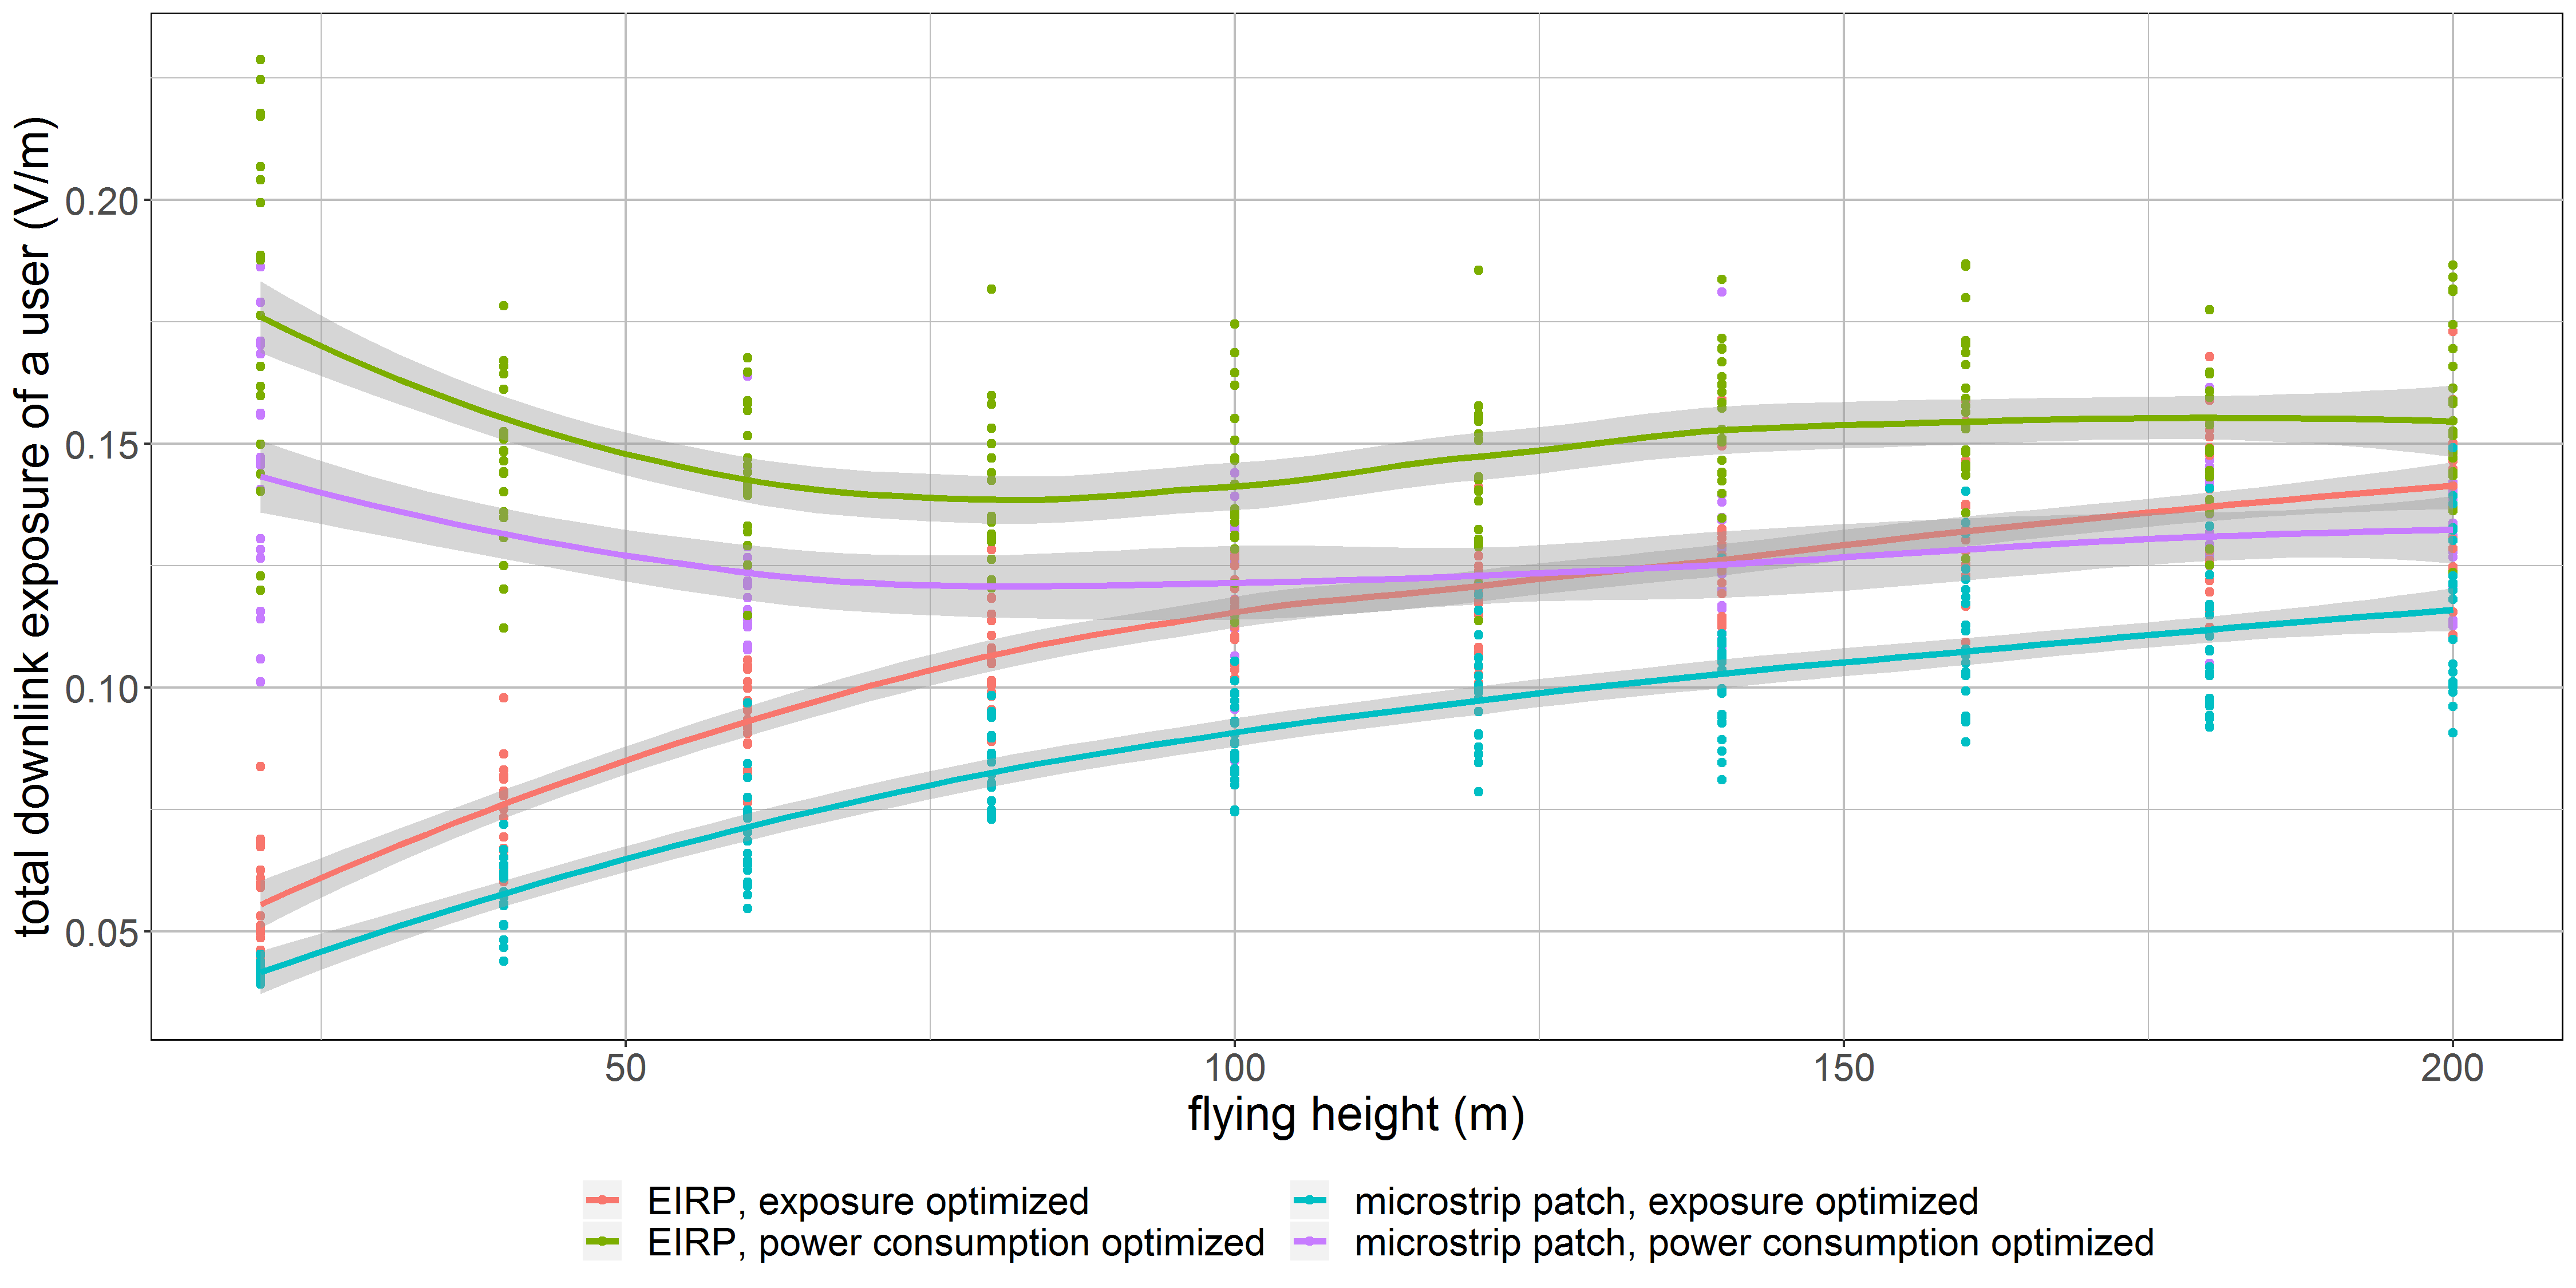
\includegraphics[width=\textwidth]{../results/s3/fhvsdl.png}
  \caption{The influence of the flying height on the downlink electromagnetic radiation of the average user.}
  \label{fig:s3fhvsdl}
\end{figure}

\begin{figure}[]
  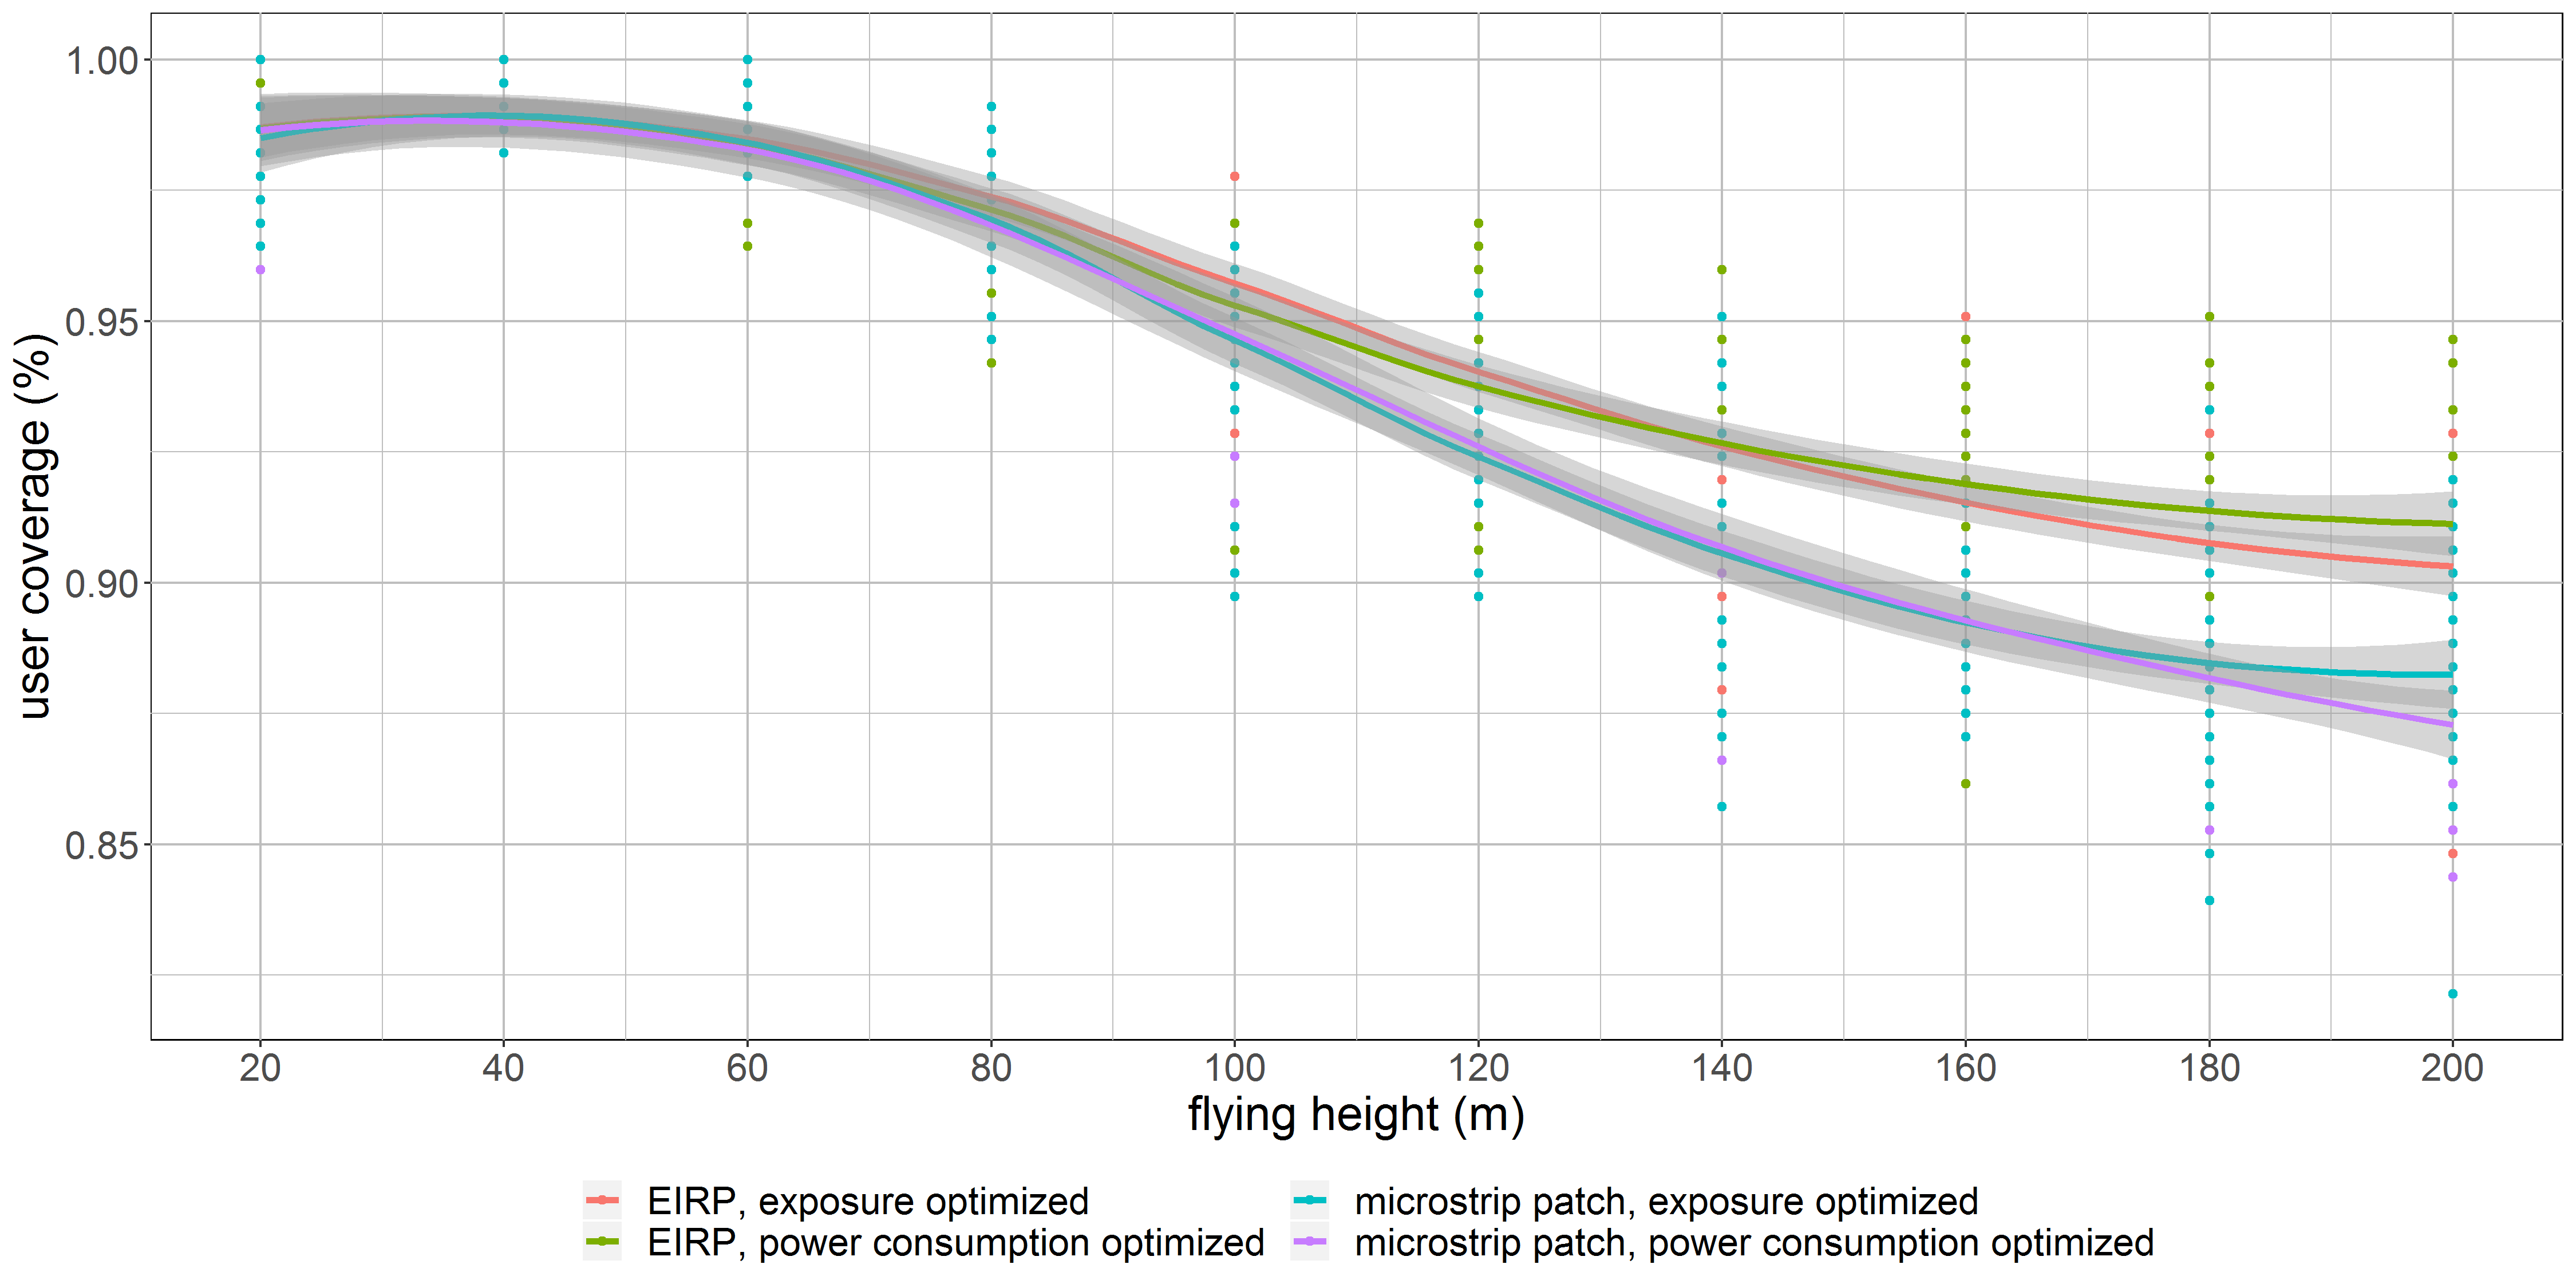
\includegraphics[width=\textwidth]{../results/s3/fhvscov.png}
  \caption{This graph shows the percentage of covered users by one drone for different flying heights.}
  \label{fig:s3fhvscov}
\end{figure}

\begin{figure}[]
  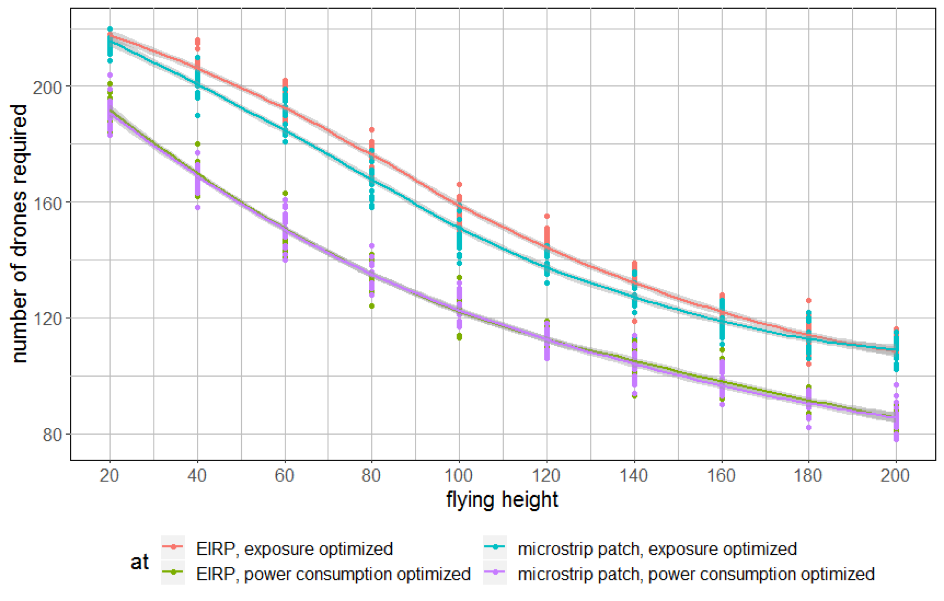
\includegraphics[width=\textwidth]{../results/s3/fhvsnumdrones.png}
  \caption{This graph shows how much drones are required for different flying heights while trying to achieve a 100\% coverage.}
  \label{fig:s3fhvscov}
\end{figure}

\begin{figure}[h!]
  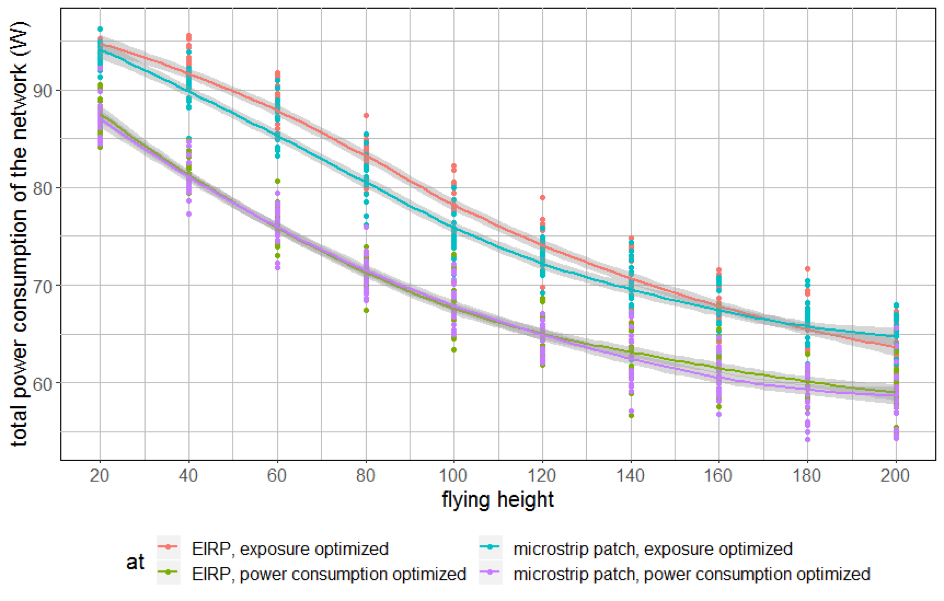
\includegraphics[width=\textwidth]{../results/s3/fhvspc.png}
  \caption{The influence of the flying height on the total power consumption of the network.}
  \label{fig:s3fhvspc}
\end{figure}

Both \ref{fig:s3fhvsnumdrones} and \ref{fig:s3fhvspc} show that the network profit from increasing the flying altitude. 
Not only less drones are needed but also the power consumption is lower. Both can be explained by the lower path loss when \gls{UABS}s fly higher.
If a user cannot be covered because an \gls{UABS}s is too far away or is saturated with other users, 
the tool can simply add another \gls{UABS}. The only remaining reason that a user can’t be covered is because the position of 
the drone is obstructed by a building. The higher drones fly, the less change the position is obstructed by a building. 
In gent is this chance is zero when flying higher then 119 meters. Since the `Artevelde Tower' is the highest building in Ghent.

Scenario 1 already proved that with low flying drones, the main source of electromagnetic radiation are \gls{UABS}. 
This changes around 80 meters where \gls{UL} electromagnetic radiation of the \gls{UE}
 exceeds \gls{DL} radiation in order to still be able to reach the high flying \gls{UABS}s.

\begin{figure}[]
  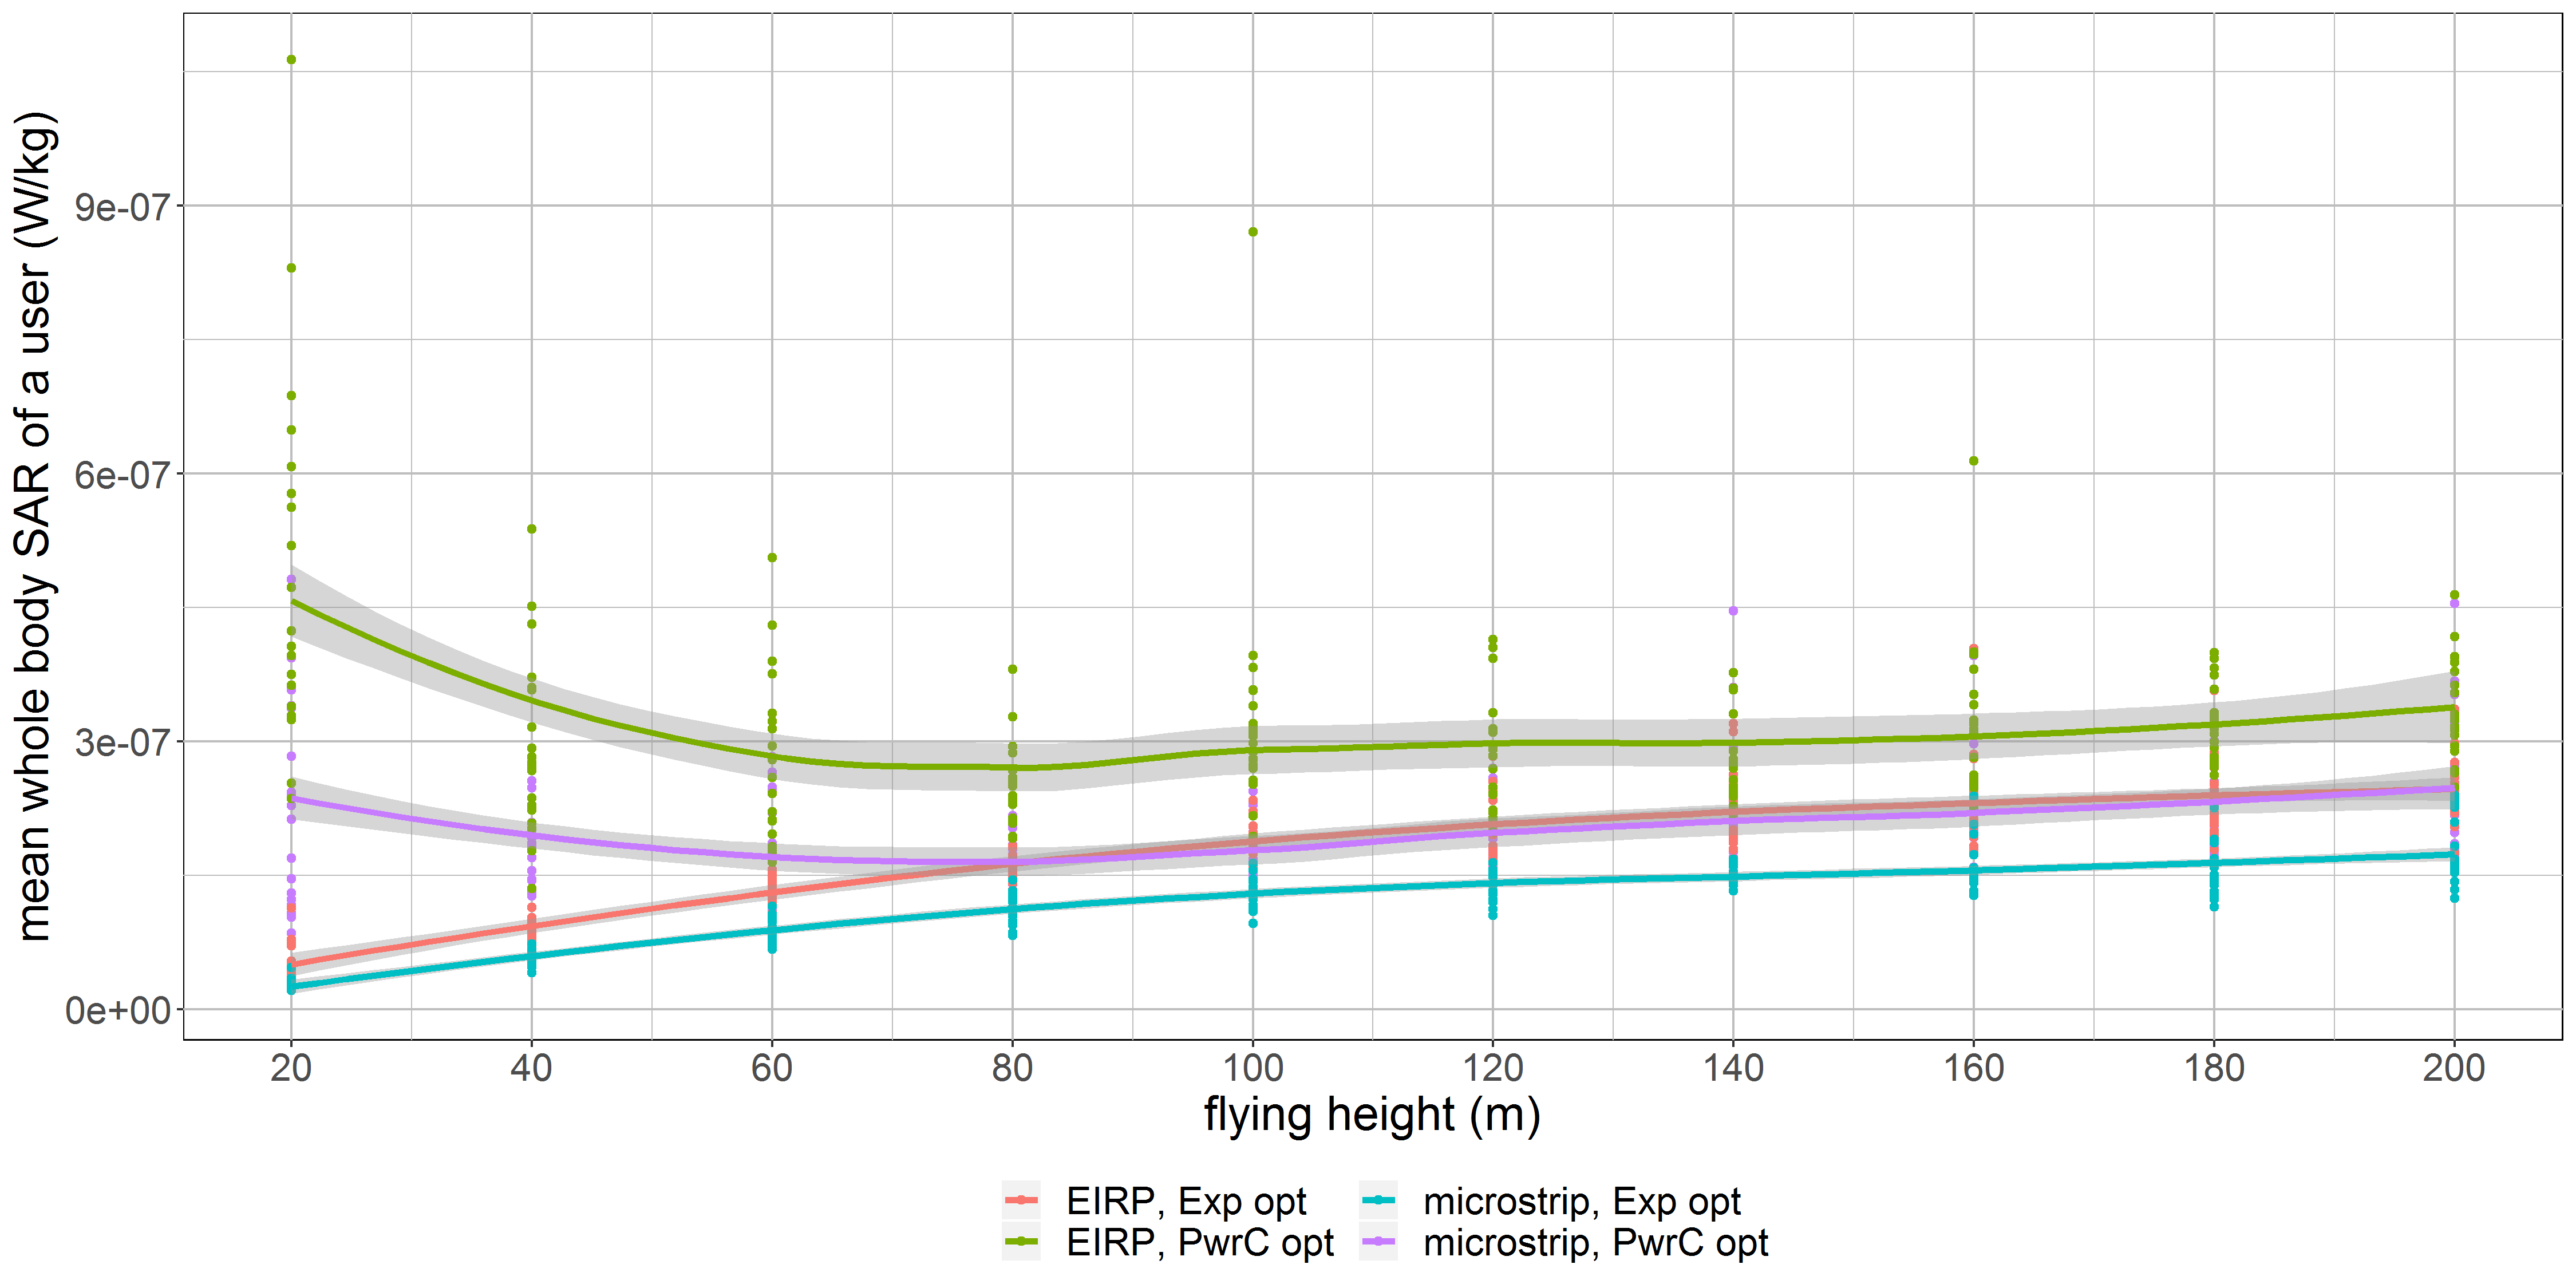
\includegraphics[width=\textwidth]{../results/s3/fhvssar.png}
  \caption{The influence of the flying height on the weighted average $SAR_{10g}$ of users in the network.}
  \label{fig:s3fhvssar}
\end{figure}

\subsection{Influence of the number of users}
todo